\documentclass{homework}

\usepackage{longtable} % para tablas largas
\usepackage{subfig}
\usepackage{multicol}
\usepackage{float}
\usepackage{bookmark}
\usepackage{hyperref}
\usepackage{xcolor}
\usepackage{listings}
\lstset{literate=
	{á}{{\'a}}1 {é}{{\'e}}1 {í}{{\'i}}1 {ó}{{\'o}}1 {ú}{{\'u}}1
	{Á}{{\'A}}1 {É}{{\'E}}1 {Í}{{\'I}}1 {Ó}{{\'O}}1 {Ú}{{\'U}}1
	{à}{{\`a}}1 {è}{{\`e}}1 {ì}{{\`i}}1 {ò}{{\`o}}1 {ù}{{\`u}}1
	{À}{{\`A}}1 {È}{{\'E}}1 {Ì}{{\`I}}1 {Ò}{{\`O}}1 {Ù}{{\`U}}1
	{ä}{{\"a}}1 {ë}{{\"e}}1 {ï}{{\"i}}1 {ö}{{\"o}}1 {ü}{{\"u}}1
	{Ä}{{\"A}}1 {Ë}{{\"E}}1 {Ï}{{\"I}}1 {Ö}{{\"O}}1 {Ü}{{\"U}}1
	{â}{{\^a}}1 {ê}{{\^e}}1 {î}{{\^i}}1 {ô}{{\^o}}1 {û}{{\^u}}1
	{Â}{{\^A}}1 {Ê}{{\^E}}1 {Î}{{\^I}}1 {Ô}{{\^O}}1 {Û}{{\^U}}1
	{ã}{{\~a}}1 {ẽ}{{\~e}}1 {ĩ}{{\~i}}1 {õ}{{\~o}}1 {ũ}{{\~u}}1
	{Ã}{{\~A}}1 {Ẽ}{{\~E}}1 {Ĩ}{{\~I}}1 {Õ}{{\~O}}1 {Ũ}{{\~U}}1
	{œ}{{\oe}}1 {Œ}{{\OE}}1 {æ}{{\ae}}1 {Æ}{{\AE}}1 {ß}{{\ss}}1
	{ű}{{\H{u}}}1 {Ű}{{\H{U}}}1 {ő}{{\H{o}}}1 {Ő}{{\H{O}}}1
	{ç}{{\c c}}1 {Ç}{{\c C}}1 {ø}{{\o}}1 {å}{{\r a}}1 {Å}{{\r A}}1
	{€}{{\euro}}1 {£}{{\pounds}}1 {«}{{\guillemotleft}}1
	{»}{{\guillemotright}}1 {ñ}{{\~n}}1 {Ñ}{{\~N}}1 {¿}{{?`}}1 {¡}{{!`}}1 
}

\definecolor{codegreen}{rgb}{0,0.6,0}
\definecolor{codegray}{rgb}{0.5,0.5,0.5}
\definecolor{codepurple}{rgb}{0.58,0,0.82}
\definecolor{backcolour}{rgb}{0.95,0.95,0.95}

\lstdefinestyle{mystyle}{
	backgroundcolor=\color{backcolour},   
	commentstyle=\color{codegreen},
	keywordstyle=\color{blue},
	numberstyle=\tiny\color{codegray},
	stringstyle=\color{codepurple},
	basicstyle=\ttfamily\footnotesize,
	breakatwhitespace=false,         
	breaklines=true,                 
	captionpos=b,                    
	keepspaces=true,                 
	numbers=left,                    
	numbersep=5pt,                  
	showspaces=false,                
	showstringspaces=false,
	showtabs=false,                  
	tabsize=2,
	xleftmargin=.25in
}

\lstset{style=mystyle}

\title{Práctica 1: Análisis de Eficiencia de Algoritmos}
\author{Shao Jie Hu Chen \\ Mario Megías Mateo \\ Jesús Samuel García Carballo}
\renewcommand{\course}{Algorítmica}
\date{1 de abril de 2022}

\begin{document}
	\maketitle

    \newpage

    \begin{abstract}
		En esta práctica hemos analizado teórica y empíricamente la eficiencia de los algoritmos de 
        ordenación de Inserción, Selección,
        QuickSort y HeapSort, así como los algoritmos de Floyd y Hanoi. Hemos creado un mecanismo para automatizar
        la generación de datos experimentales de estos algoritmos, generando automáticamente tablas y datos estadísticos
        relevantes para su análisis. También hemos comparando los diversos algoritmos de ordenación, concluyendo que
        los más eficientes son HeapSort y QuickSort, siendo el de selección el peor entre ellos. También hemos
        analizado ejecuciones con diversos niveles de optimización, concluyendo que la labor del compilador puede llegar
        a disminuir, en gran medida, el tiempo de ejecución de los algoritmos. 
	\end{abstract}
	
    \newpage

	\tableofcontents
    \newpage
    \listoftables
	\newpage
	\setcounter{page}{1}
	
	\section{Introducción}

    En esta primera práctica de la asignatura Algorítmica vamos a realizar un análisis teórico y empírico de
    diversos algoritmos vistos en la asignatura. En particular, dicho análisis se hará de los siguientes:

    \begin{itemize}
        \item \textbf{Algoritmos de ordenación:} Inserción, selección, quicksort y mergesort. 
        \item \textbf{Algoritmo de análisis de caminos mínimos sobre grafos:} Algoritmo de Floyd.
        \item \textbf{Hanoi.} Resolución del juego de las torres de Hanoi. 
    \end{itemize}

    \subsection{Estructura de la memoria}
    
	Esta memoria presenta la estructura típica de un trabajo académico. En primer lugar, presentamos
    brevemente el contexto en el que nos manejamos en esta práctica. Posteriormente, analizaremos teóricamente
    cada uno de los algoritmos propuestos para, seguidamente, comprobar mediante un 
    análisis empírico las soluciones obtenidas. Asimismo, se ha realizado un análisis híbrido contrastando
    los resultados teóricos con los experimentales. Este análisis se ha realizado para cada algoritmo, 
    extrayéndose información relevante asociada a ellas. 
    
    Además, para cada uno de los algoritmos considerados, se ha
    elaborado conjuntamente entre los miembros del grupo tablas asociadas a cada una de ellas, que se
    irán presentando a lo largo de esta memoria. Finalmente, se escribirán unas
    líneas asociadas a las conclusiones obtenidas tras el desarrollo de esta práctica, así como los resultados
    más relevantes obtenidos. 

    \subsection{Objetivos} 

    Entre los objetivos que vamos a realizar asociadas a esta práctica, caben destacar los siguientes: 

    \begin{itemize}
        \item \textbf{Estudio teórico, empírico e híbrido} y \textbf{comparación} de los algoritmos de ordenación más empleados, verificando los resultados teóricos.
        \item \textbf{Estudio teórico, empírico e híbrido} de algoritmos de alta complejidad, poniendo especial énfasis en su \textbf{viabilidad} en diferentes equipos. 
        \item Estudio del \textbf{aumento de eficiencia} de un mismo algoritmo para diferentes \textbf{tipos de optimización} del compilador. 
        \item Determinación del algoritmo \textbf{más adecuado} para cada situación en función del estado de los datos.
    \end{itemize}

    \subsection{Equipo empleado}

    Para el desarrollo de esta práctica, se han empleado diferentes equipos, cuyas respectivas especificaciones técnicas se 
    especifican a continuación:
    
    \begin{itemize}
        \item \textbf{ASUS} 
        \begin{itemize}
            \item \textbf{Modelo}: ZenBook 15 UX534F
            \item \textbf{Procesador}: Intel(R) Core(TM) i7-10510U CPU @ 1.80GHz5
            \item \textbf{Memoria Ram}: 16 GB DDR4 @ 2.133 MHz.
            \item \textbf{Sistema Operativo} Ubuntu 20.04.2 LTS
        \end{itemize}
        
        \item \textbf{LENOVO}
        \begin{itemize}
            \item \textbf{Modelo}: YOGA 530-14IKB
            \item \textbf{Procesador}: Intel(R) Core(TM) i5-8250U CPU @ 1.60GHz
            \item \textbf{Memoria RAM:} 8 GB DDR4
            \item \textbf{Sistema Operativo}: Ubuntu 20.04.4 LTS
        \end{itemize}
        
        \item \textbf{HP}
        \begin{itemize}
            \item \textbf{Modelo}: Pavilion Gaming Laptop 15-dk0xxx
            \item \textbf{Procesador}: Intel(R) Core(TM) i7-9750H CPU @ 2.60GHz
            \item \textbf{Memoria RAM:} 32 GB DDR4
            \item \textbf{Sistema Operativo}: Ubuntu 20.04.4 LTS
        \end{itemize}
    \end{itemize}
    
    \newpage
    \section{Metodología}

    Debido a las limitaciones técnicas de estos equipos, para el cálculo de la eficiencia empírica se ha 
    optado por medir tiempos de ejecución en tiempos y \textbf{tamaños razonables} para obtener datos relevantes
    para el comportamiento tanto a pequeñas escalas como a nivel asintótico de ellas. 

    Con el fin de automatizar el desarrollo de esta práctica, se ha diseñado un proyecto a la que hemos llamado 
    \textbf{GraphKiller}. Se trata de un conjunto de 6 scripts cuya última finalidad es la de automatizar la generación
    de los parámetros que aparecen en este práctica. Un esquema de este proyecto puede encontrar en la 
    figura \ref{graph-killer}. 

    \begin{figure}[H]
        \centering
        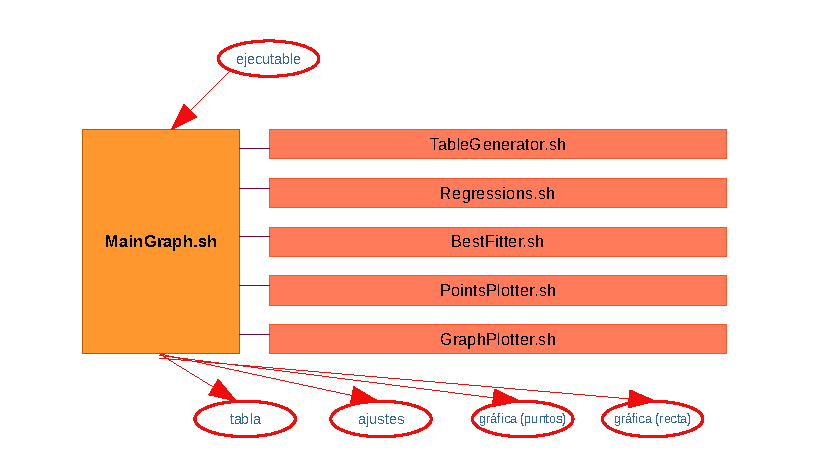
\includegraphics[width=0.87\textwidth]{img/esquema_graphkiller.pdf}
        \caption{Esquema del funcionamiento de GraphKiller}
        \label{graph-killer}
    \end{figure}

    Consta de las siguientes partes:

    \begin{enumerate}
        \item \textbf{TableGenerator.sh}. Se encarga de generar las tablas de datos, teniendo en cuenta número de repeticiones, valores iniciales y finales y cantidad de medidas experimentales a tomar.
        \item \textbf{Regressions.sh}. Se encarga de generar una lista de las regresiones más empleadas en Algorítmica, dando información como función de ajuste y parámetros estadísticos como la varianza residual de la regresión.
        \item \textbf{BestFitter.sh}. Su labor es la de escoger siempre la regresión que mejor se ajusta (con menor varianza residual). Presenta el inconveniente de que no sabe discriminar los datos, únicamente compara residuos.
        \item \textbf{PointsPlotter.sh}. Produce un gráfico con los puntos de la tabla de datos obtenida.
        \item \textbf{GraphPlotter.sh}. Produce un gráfico con los puntos de la tabla de datos obtenida, así como la curva de regresión óptima. 
        \item \textbf{MainGraph.sh}. Es el guión que articula todos los anteriores. Es el encargado de recibir el ejecutable de un programa y organizar todos los datos y gráficos en la jerarquía de archivos. 
    \end{enumerate}

    Además para poder ejecutar toda la información pedida para unos ciertos valores, los cuales varían para los de ordenación, Floyd y Hanoi, hemos decidido crear un script que directamente
    ejecute el MainGraph, imponiendo que cada algoritmo se ejecute según los valores expuestos. 

    De esta manera, ha sido fácil ponernos de acuerdo en ejecutar los mismos valores, porque únicamente había que ejecutar
    los scripts que habíamos elaborado, eliminado el factor de error humano.  
    
    En conclusión este script sería como nuestra pólvora que al ejecutarlo nos daría las gráficas, tablas y mejor regresión de cada algoritmo.
    
    \newpage
    \section{Eficiencia teórica}

    Para el análisis de los siguientes algoritmos se ha empleado la notación $O(.)$. 

    \subsection{Algoritmo HeapSort}
    
    \lstinputlisting[language=C++, firstline=56, lastline=68, caption=Implementación en C++ del algoritmo heapsort.]{../src/heapsort.cpp} 

    El heapsort es un algoritmo de ordenación por montículos que consta de dos bucles for independientes, que llaman a una función llamada reajustar.
    En la primera línea de código podemos encontrar una declaración de variable cuya eficiencia es $O(1)$ y luego los dos ciclos mencionados, que interan 
    sobre el número de elementos del vector que denotaremos por $n$, luego realizaremos la eficiencia en torno a este dato. Ambos ciclos son independientes, 
    así que vamos a analizar cada uno por separado y aplicando la regla del máximo nos quedaremos con el mayor.
    
    La función reajustar trata de imitar el uso de un árbol APO mediante vectores y recorrerlo insertando elementos, luego como en un árbol APO la inserción se 
    realiza con eficiencia $O(log_2(n))$. Así que llamando $T(n)$ al números de operaciones asociadas al algoritmo, tenemos lo siguiente:
    
    \begin{itemize}
        \item \textbf{Primer ciclo}
        \begin{equation*}
            T(n) = \sum_{i=1}^{n/2 + 1} \log_2(i) = \log_2((n/2 + 1)!) \leq (n/2+1) \cdot log(n/2+1) \in O(nlog_2(n))
        \end{equation*} 

        \item \textbf{Segundo ciclo}
            $$\sum_{i=1}^{n-1} \log_2(i) = \log_2(2) + ... + \log_2(n-1) = \log_2((n-1)!) \leq (n-1) \cdot log(n-1) \in O(n \log_2(n))$$
        
        
    \end{itemize}

    En conclusión vemos que como tenemos que aplicar la regla del máximo y ambos ciclos tienen de eficiencia $O(nlog(n))$ podemos afirmar que esa es la eficiencia
    teórica del algoritmo. 

    \subsection{Algoritmo QuickSort}
    
    \lstinputlisting[language=C++, firstline=141, lastline=184, caption=Implementación en C++ del algoritmo QuickSort.]{../src/quicksort.cpp} 

    En este apartado, consideramos $n$ como el número de componentes del vector. 

    El código del algoritmo comienza en la función quicksort\_lims en la línea 6. Tomaremos inicial 
    como posición inicial del vector (inicial = $0$), y final como el siguiente al último elemento, 
    que coincide con el número de componentes del vector (final = $n$).
    
    Tenemos una estructura condicional que determina el comportamiento del algoritmo según si el tamaño del vector 
    supera o no un cierto umbral, por lo que el tiempo de ejecución será una función definida a trozos. Si es menor 
    que el umbral, ejecutamos la ordenación con el algoritmo de inserción previamente analizado, que es $O(n^2)$. De lo
    contrario, realizamos la ordenación según el propio algoritmo quicksort. Dicho algoritmo se basa en la técnica de Divide
    y Vencerás, implementándose de forma recursiva. 
    
    En primer lugar, se realiza una llamada a la función dividir dividir\_qs, 
    cuya eficiencia procedemos a analizar. En las líneas 24-26 y 40-43 tenemos sentencias de asignación que serán despreciadas. 
    Siguiendo código de forma secuencial, en las líneas 27 y 30 tenemos dos bucles do-while, si consideramos el peor caso para 
    el primero (el pivote es mayor que el resto de elemento) tiene eficiencia $O(n)$, y el caso contrario al anterior sería el 
    más desfavorable para el segundo (el pivote es menor que el resto de los elementos), luego tendríamos $O(n)$. 
    
    Como el caso más 
    favorable para uno (eficiencia $O(1)$) es el más desfavorable para el otro, aplicando la regla del Máximo tenemos que la 
    eficiencia de la parte del código de los do-while sería $O(n)$.  A continuación, encontramos un bucle while que se ejecuta un 
    número indeterminado de veces en función de la condición, luego podemos acotar estas ejecuciones por una constante c. En las 
    líneas 34-36 tenemos sentencias de asignación que serán ignoradas, y a continuación dos bucles do-while con la misma funcionalidad
    que los analizados anteriormente. 
    
    Por tanto, deducimos que la eficiencia del bucle while es $O(n)$, y aplicando la regla del 
    Máximo con el bloque de código de los bucles do-while obtenemos que la eficiencia de la función es $O(n)$. A continuación hacemos dos llamadas
    recursivas, una que procesará los datos desde el comienzo del mismo hasta la posición en la que hemos ubicado el pivote con la 
    función dividir\_qs, y la otra se encarga de procesar el resto del vector. Por tanto, el tiempo de ejecución sería:

    \begin{equation}
        T(n) = \left\{ \begin{array}{lr} T(k_n) + T(n-k_n) + n & \text{si } n \geq \text{UMBRAL}\\ n^2 & \text{si } n < \text{UMBRAL} \end{array} \right.
    \end{equation}

    Para el caso promedio, podemos considerar que $k_{n} = \frac{n}{2}$. Resolvamos la recurrencia de (1):
    
    \begin{equation}
        T(n) = T(k_n) + T(n-k_n) + n \text{ si n $\geq$ UMBRAL}
    \end{equation}

    Realizamos el cambio de variable $n = 2^{n}$ en la ecuación (2) obtenemos:

    \begin{equation}
        T(2^{m}) = 2T(2^{m-1}) + 2^{m} \text{ si n $\geq log_{2}$(UMBRAL)} 
    \end{equation}

    \begin{equation}
        T(2^{m}) - 2T(2^{m-1}) = 2^{m}
    \end{equation}

    Renombramos la expresión anterior como $T(2^{m}) = t_{m}$ obtenemos:

    \begin{equation}
        t_{m} - 2t_{m-1} = 2^{m}
    \end{equation}
    
    Obtenemos la siguiente ecuación de recurrencia de la ecuación (5):

    \begin{equation}
        (x-2)^{2} = 0
    \end{equation}

    Luego la solución general de la recurrencia es:

    \begin{equation}
        t_{m} = c_{1}2^{m} + c_{2}m2^{m}
    \end{equation}

    Deshacemos el cambio de variable:

    \begin{equation}
        T(n) = c_{1}n + c_{2}nlog_{2}(n)
    \end{equation}

    Por tanto $T(n) \in O(nlog_{2}(n))$ si n $\geq$ UMBRAL.

    \subsection{Algoritmo de inserción}

    El código de este algoritmo lo podemos encontrar a continuación.

    \lstinputlisting[language=C++, firstline=66, lastline=79, caption=Implementación en C++ del algoritmo de inserción.]{../src/insercion.cpp}
    
    El análisis de eficiencia se ha de hacer sobre el número de elementos del vector $n$. 

    Para el análisis asintótico, calculamos el número de operaciones elementales asociadas al código. 
    Las tres primeras líneas tienen complejidad $O(1)$. Para el ciclo for, démonos cuenta de que itera sobre el número de
    componentes del vector. Por su parte, dentro del for existe un while que realiza un conjunto de operaciones de orden
    $O(1)$ tantas veces como se indica en el iterador. Por tanto, llamando $T(n)$ al números de operaciones asociadas
    al algoritmo, tenemos que:

    \begin{equation*}
        T(n) = \sum_{i=0}^{n-1} \sum_{j=0}^{i-1} k = \sum_{i=0}^{n-1} ki = k \frac{n(n-1)}{2} 
    \end{equation*}

    Por tanto, deducimos que $T(n) \in O(n^2)$. 

    \subsection{Algoritmo de selección}

    \lstinputlisting[language=C++, firstline=66, lastline=82, caption=Implementación en C++ del algoritmo de selección.]{../src/seleccion.cpp}    

    La estructura principal del código anterior consta de dos bucles for anidados. Las primeras sentencias de declaración antes del inicio del primer 
    bucle for no repercuten en el análisis. Procedamos a analizar la estructura repetitiva: el primer for recorre el vector desde su inicio hasta
    la penúltima componente del mismo incluída. El segundo for comienza en la posición dada por el índice del primero hasta la última componente del vector incluída.
    Dentro del bucle interno tenemos una operación elemental correspondiente a la comparación realizada en el if, que es $O(1)$. Dentro del bucle externo excluyendo 
    el código del bucle interno nos encontramos con dos sentencias de asignación que no se tendrán en cuenta para el análisis. De igual modo, fuera del bucle externo
    al final del código nos encontramos con otras sentencias de asignación que también serán despreciadas. También tendremos en cuenta las operaciones elementales
    aritméticos correspondientes a la gestión de los bucles, que son $O(1)$. En conclusion, acotando las expresiones $O(1)$ por k tenemos que: 

    \begin{equation*}
        \begin{split}
            T(n) = \sum_{i=0}^{n-2} \sum_{j=i}^{n-1} k = \sum_{i=0}^{n-2} k(n-1-i+1) = \sum_{i=0}^{n-2} k(n-i) = kn \sum_{i=0}^{n-2} 1  - k \sum_{i=0}^{n-2} i \\
            = kn(n-2+1) - k \frac{(n-2)(n-1)}{2} = kn^2 + kn - \frac{kn^2 - 3kn + 2k}{2}
        \end{split}
    \end{equation*}
    
    Deducimos, por tanto, que $T(n) \in O(n^2)$. 
    
    \subsection{Algoritmo de Floyd}

    A continuación se presenta el código de este algoritmo:

    \lstinputlisting[language=C++, firstline=129, lastline=138, caption=Implementación en C++ del algoritmo de Floyd.]{../src/floyd.cpp}

    En este caso, consideramos como $n$ el número de filas/columnas de la matriz. Como los tres bucles iteran cada uno sobre n, siendo el número de iteraciones
    independientes entre sí y se realizan $k$ operaciones en cada una de ellas, tenemos que llamando $T(n)$ al número de operaciones para un tamaño n, se verifica:
    
    \begin{equation*}
        T(n) = \sum_{i=1}^n \sum_{j=1}^{n} \sum_{k=1}^{n} k = kn^3
    \end{equation*}

    Deducimos fácilmente que $T(n) \in O(n^3)$. 
    
    \vspace{2em}

    \subsection{Algoritmo Hanoi}
    
    \lstinputlisting[language=C++, firstline=30, lastline=38, caption=Implementación en C++ del algoritmo de resolución de las torres de Hanoi.]{../src/hanoi.cpp} 

    Estamos ante el estudio de un algoritmo recursivo, así que si T(n) es el número de movimientos necesarios para mover n discos, tenemos que el algoritmo sigue la 
    recurrencia $T(n) = 2T(n-1) + 1$ $\forall n \geq 1$ y con $T(0) = 0$ como caso base. Por lo tanto, vamos a resolverla para hallar su eficiencia teórica.

    Tenemos que $t_n - 2t_{n-1} = 1 $ luego si hacemos un cambio de varible nos queda como ecuación característica $(x-2)(x-1) = 0$, que son las propias raíces de la 
    recurrencia luego la solución nos queda $t_n = c_1 1^n  + c_2 2^n  $. Como $t_0=0$, nos sale que $t_0 = c_1 + c_2$ y $t_1 = 2 t_0 + 1 = 1$, luego en la 
    solución $t_1=c_1 + 2 c_2 $, de donde si resolvemos el sistema $c_1 = 1$ y $c_2 = -1$ nos queda la ecuación $2^n - 1^n$. 
    
    En consecuencia, deducimos que se trata de la ecuación que 
    modela la recurrencia, lo que nos permite concluir que la eficiencia teórica del algoritmo es $O(2^n)$.

    \newpage
    \section{Eficiencia empírica}

    Para esta práctica hemos ejecutado en cada uno de los equipos un algoritmo de cada orden de eficiencia.
    Las tablas obtenidas, así como las gráficas correspondientes se representan a continuación.

    Las tablas de los siguientes epígrafes presentan las siguientes características:

    \begin{itemize}
        \item La \textbf{primera columna} es el parámetro respecto al cual se busca la eficiencia del algoritmo.
        \item La columna $t_{ASUS}$ indica el tiempo, en $\mu$s, empleado para ejecutar el algoritmo para el tamaño considerado por el equipo Asus.
        \item La columna $t_{HP}$ indica el tiempo, en $\mu$s, empleado para ejecutar el algoritmo para el tamaño considerado por el equipo HP.
        \item La columna $t_{LENOVO}$ indica el tiempo, en $\mu$s, empleado para ejecutar el algoritmo para el tamaño considerado por el equipo Lenovo.
    \end{itemize}
    
    En lo que sigue hemos adaptado el mismo orden en todas las tablas, con la finalidad de facilitar su lectura. Las columnas
    han sido organizadas de forma alfabética, de forma que se pueda localizar de forma aún más rápida. Además,este orden coincide con la potencia de nuestros procesadores,
    siendo el de más rápido el ASUS y el más lento el Lenovo.

    Asimismo, hemos expuesto cada algoritmo en dos páginas, la primera que consta fundamentalmente de la tabla y
    de algunas conclusiones y en la segunda se presentan las gráficas experimentales representando los puntos
    obtenidos tras la ejecución de GraphKiller. 

    Las gráficas se han obtenido mediante la herramienta Gnuplot. Para algunas de ellas también se ha empleado un script
    para automatizar la generación de ellas, si bien es cierto que hay algunas que, por no ser tan rutinarias y requerir
    de una única ejecución, se ha optado por realizarlo directamente en la terminal que se muestra para ejecutar gnuplot.

    \newpage

    \subsection{Algoritmo QuickSort}

    Empezamos analizando el algoritmo de menor orden de complejidad. La tabla con los valores obtenidos de la ejecución
    de cada algoritmo con sus respectivos tiempos de ejecución se pueden observar a continuación.

    En la siguiente tabla se encuentran los datos obtenidos en este algoritmo por cada uno de los
    equipos en los que hemos ejecutado el algoritmo. 

    \begin{table}[h]
        \footnotesize
        \centering
            \begin{tabular}{|r|r|r|r|}
                \hline
                \text{$N_{componentes}$} & \text{$t_{ASUS}$} & \text{$t_{HP}$} & \text{$t_{LENOVO}$} \\
                \hline
                50 & 0.17 & 0.52 & 0.35 \\ 
                1550 & 6.61 & 6.61 & 15.56 \\ 
                3050 & 14.03 & 12.35 & 39.12 \\ 
                4550 & 22.15 & 17.27 & 39.49 \\ 
                6050 & 30.74 & 23.82 & 61.13 \\ 
                7550 & 39.04 & 34.79 & 64.00 \\ 
                9050 & 46.95 & 36.57 & 67.17 \\ 
                10550 & 56.34 & 40.18 & 77.66 \\ 
                12050 & 71.14 & 50.55 & 90.32 \\ 
                13550 & 89.81 & 55.28 & 101.90 \\ 
                15050 & 88.45 & 61.57 & 119.67 \\ 
                16550 & 98.56 & 70.63 & 134.65 \\ 
                18050 & 107.69 & 75.28 & 145.62 \\ 
                19550 & 117.73 & 80.04 & 150.02 \\ 
                21050 & 127.28 & 85.59 & 163.49 \\ 
                22550 & 117.67 & 90.47 & 175.83 \\ 
                24050 & 115.74 & 100.66 & 187.89 \\ 
                25550 & 129.62 & 110.87 & 205.24 \\ 
                27050 & 130.34 & 117.50 & 214.19 \\ 
                28550 & 137.97 & 123.90 & 228.24 \\ 
                30050 & 147.05 & 131.77 & 245.48 \\ 
                31550 & 191.97 & 137.76 & 254.54 \\ 
                33050 & 191.03 & 142.09 & 269.09 \\ 
                34550 & 192.52 & 153.92 & 281.52 \\ 
                36050 & 197.37 & 160.30 & 299.20 \\ 
                37550 & 210.15 & 167.35 & 326.10 \\ 
                39050 & 219.80 & 170.98 & 329.71 \\ 
                40550 & 231.73 & 180.96 & 336.20 \\ 
                42050 & 238.25 & 188.74 & 346.37 \\ 
                43550 & 262.80 & 200.55 & 358.76 \\ 
                \hline
            \end{tabular}
        \caption{Tiempos de ejecución (en $\mu$s) del algoritmo de QuickSort}
    \end{table}

    Así que como preveíamos, puesto que habíamos estudiado las características del hardware de cada ordenador, hemos visto que el ASUS al 
    tener un i7 de 10ª generación ejecuta más rápido el algoritmo que el resto, mientras que el LENOVO es el computador que más tarda, 
    lógicamente al tratarse de un i5, y el HP con un i7 de 9º generación, que se correspondería con el equipo de nivel intermedio, tiene unos tiempos
    de ejecución levemente superiores al ASUS.  
    
    Ahora vamos a mostrar las gráficas resultantes tras calcular el tiempo que tarda la ejecución de este algoritmo para diferentes
    tamaños, en este caso, para distintos tamaños del vector.

    \begin{figure}[H]
        \centering
         \subfloat[ASUS]{
          \label{asus:quicksort-emp}
           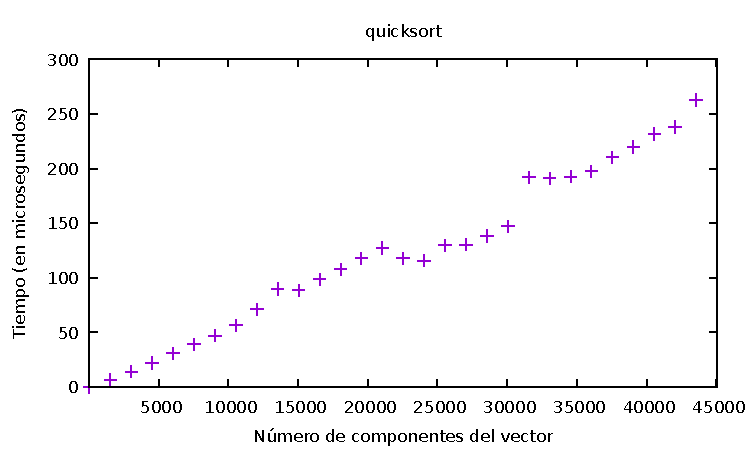
\includegraphics[width=0.7\textwidth]{../data/asus/quicksort-points.pdf}}

         \subfloat[HP]{
          \label{hp:quicksort-emp}
           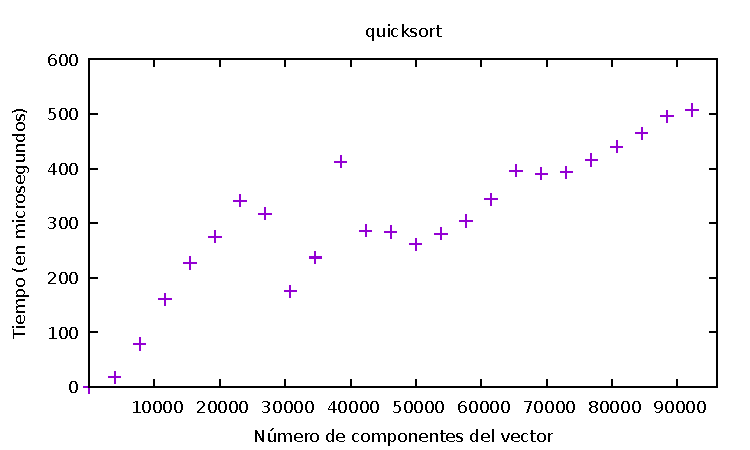
\includegraphics[width=0.7\textwidth]{../data/hp/quicksort-points.pdf}}

         \subfloat[LENOVO]{
          \label{lenovo:quicksort-emp}
           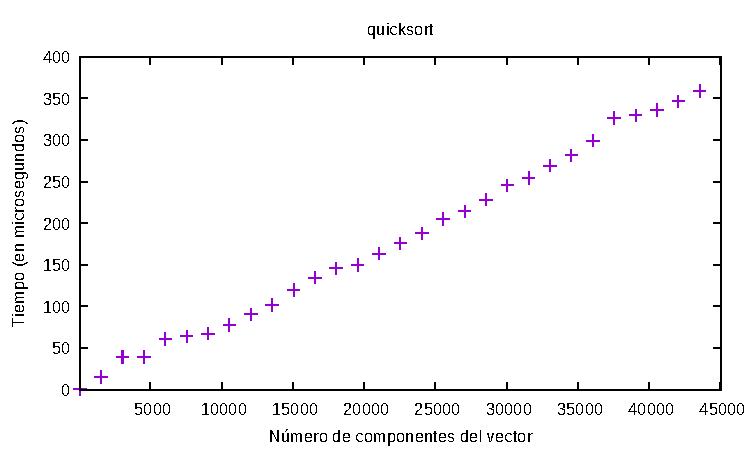
\includegraphics[width=0.7\textwidth]{../data/lenovo/quicksort-points.pdf}}
        \caption{Representación gráfica de tiempos de ejecución del algoritmo de ordenación QuickSort.}

        \label{emp:quicksort}
    \end{figure}

    \newpage
    
    \subsection{Algoritmo de inserción}
    
    En la siguiente tabla se encuentran los datos obtenidos en este algoritmo por cada uno de los
    equipos en los que hemos ejecutado el algoritmo. 
    
    \begin{table}[h]
        \footnotesize
        \centering
        \begin{tabular}{|r|r|r|r|}
            \hline
            \text{$N_{componentes}$} & \text{$t_{ASUS}$} & \text{$t_{HP}$} & \text{$t_{LENOVO}$} \\
            \hline
            50 & 0.20 & 0.18 & 0.32 \\ 
            1550 & 75.77 & 165.44 & 113.40 \\ 
            3050 & 256.80 & 378.04 & 416.61 \\ 
            4550 & 568.78 & 586.46 & 818.87 \\ 
            6050 & 1009.34 & 1038.65 & 1318.29 \\ 
            7550 & 1563.83 & 1571.11 & 2040.42 \\ 
            9050 & 2223.38 & 2257.82 & 2893.16 \\ 
            10550 & 3041.16 & 3038.05 & 3937.94 \\ 
            12050 & 3990.62 & 3987.64 & 5111.43 \\ 
            13550 & 5006.11 & 5034.40 & 6412.50 \\ 
            15050 & 6150.48 & 6111.62 & 7911.75 \\ 
            16550 & 7465.37 & 7329.81 & 9605.05 \\ 
            18050 & 8826.78 & 8700.77 & 11396.08 \\ 
            19550 & 10378.18 & 10203.49 & 13402.47 \\ 
            21050 & 11990.83 & 11768.61 & 15511.25 \\ 
            22550 & 13870.88 & 13507.03 & 17763.31 \\ 
            24050 & 15767.71 & 15368.75 & 20213.18 \\ 
            25550 & 17623.01 & 17377.42 & 22797.11 \\ 
            27050 & 19843.40 & 19877.53 & 25575.44 \\ 
            28550 & 22034.17 & 22049.19 & 28426.29 \\ 
            30050 & 24340.38 & 24031.41 & 31521.96 \\ 
            31550 & 27098.83 & 26888.22 & 34782.56 \\ 
            33050 & 29862.88 & 29816.95 & 38191.71 \\ 
            34550 & 32503.73 & 32544.47 & 41713.63 \\ 
            36050 & 35181.93 & 34468.33 & 45353.92 \\ 
            37550 & 38327.38 & 38378.51 & 49245.56 \\ 
            39050 & 41369.21 & 41678.47 & 53230.43 \\ 
            40550 & 44358.82 & 44103.68 & 57379.06 \\ 
            42050 & 48124.07 & 47379.56 & 61712.14 \\ 
            43550 & 51624.04 & 50204.90 & 66215.14 \\ 
            \hline
        \end{tabular}
        \caption{Tiempos de ejecución (en $\mu$s) del algoritmo de inserción}
    \end{table}

    Tal y como podemos observar, tenemos que nuevamente el equipo de ASUS ofrece un \textbf{mejor rendimiento} respecto a los otros
    dos equipos en los que se ha realizado el análisis. Asimismo, el tiempo de ejecución aumenta considerablemente
    en cuanto el número de componentes de vector en comparación con los algoritmos de QuickSort o MergeSort. 

    \begin{figure}[h]
        \centering
        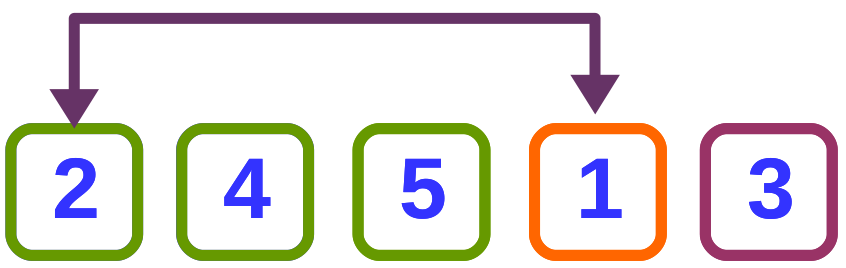
\includegraphics[width=0.5\textwidth]{img/insercion.png}
        \caption{Ilustración del funcionamiento interno del algoritmo de inserción}
    \end{figure}

    Las gráficas asociadas a cada equipo se pueden encontrar a continuación:

    \begin{figure}
        \centering
         \subfloat[ASUS]{
          \label{asus:insercion-emp}
           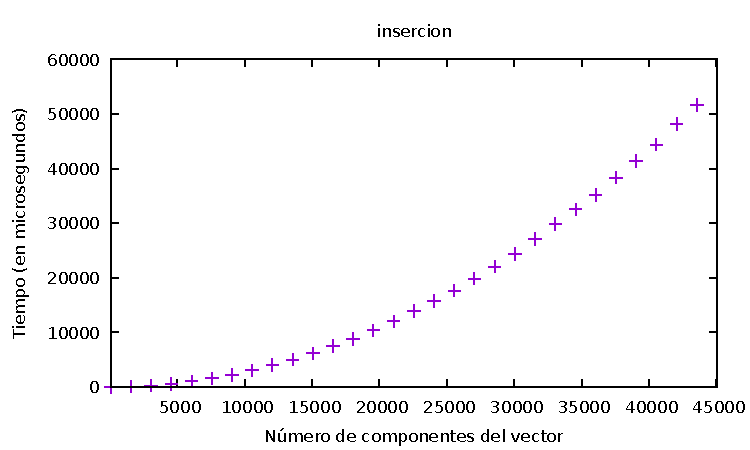
\includegraphics[width=0.7\textwidth]{../data/asus/insercion-points.pdf}}

         \subfloat[HP]{
          \label{hp:insercion-emp}
           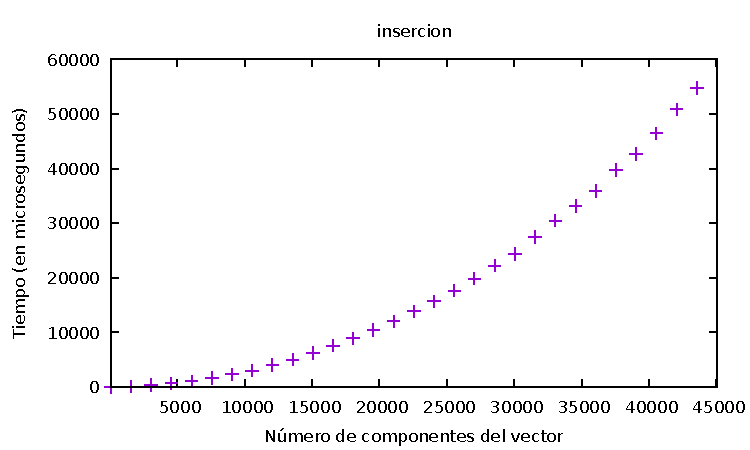
\includegraphics[width=0.7\textwidth]{../data/hp/insercion-points.pdf}}

         \subfloat[LENOVO]{
          \label{lenovo:insercion-emp}
           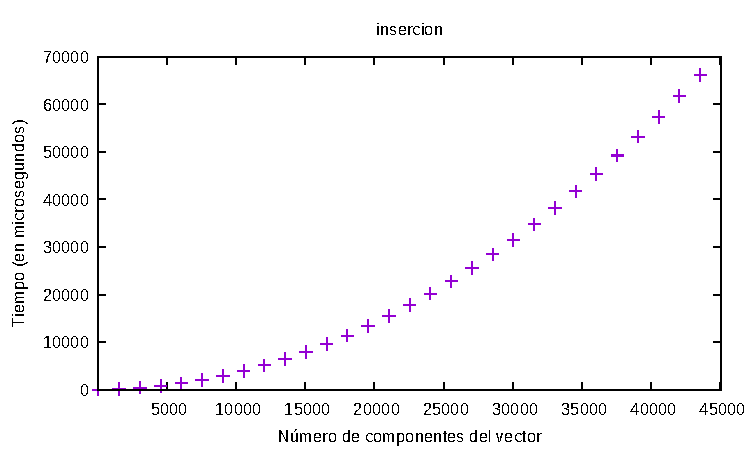
\includegraphics[width=0.7\textwidth]{../data/lenovo/insercion-points.pdf}}
        \caption{Representación gráfica de tiempos de ejecución del algoritmo de inserción.}

        \label{emp:insercion}
    \end{figure}
    
    \newpage 
    
    \subsection{Algoritmo de Floyd}

    En la siguiente tabla se encuentran los datos obtenidos en este algoritmo por cada uno de los
    equipos en los que hemos ejecutado el algoritmo. 

    \begin{table}[H]
        \centering
        \begin{tabular}{|r|r|r|r|}
            \hline
            \text{$N_{nod}$} & \text{$t_{ASUS}$} & \text{$t_{HP}$} & \text{$t_{LENOVO}$} \\
            \hline
            5 & 0.09 & 0.10 & 0.13 \\ 
            35 & 4.63 & 5.04 & 3.79 \\ 
            65 & 28.11 & 36.27 & 22.68 \\ 
            95 & 98.97 & 59.42 & 76.20 \\ 
            125 & 206.65 & 291.02 & 171.84 \\ 
            155 & 250.74 & 340.20 & 294.25 \\ 
            185 & 368.58 & 490.17 & 466.89 \\ 
            215 & 572.04 & 588.29 & 727.49 \\ 
            245 & 846.54 & 873.17 & 1069.24 \\ 
            275 & 1193.13 & 1234.56 & 1530.57 \\ 
            305 & 1642.20 & 1666.67 & 2058.39 \\ 
            335 & 2164.11 & 2205.70 & 2755.76 \\ 
            365 & 2826.06 & 2846.01 & 3574.31 \\ 
            395 & 3528.34 & 3583.40 & 4484.65 \\ 
            425 & 4410.26 & 4465.64 & 5606.11 \\ 
            455 & 5383.56 & 5485.51 & 6820.05 \\ 
            485 & 6554.77 & 6483.90 & 8154.31 \\ 
            515 & 7855.67 & 7928.90 & 9760.62 \\ 
            545 & 9386.40 & 9268.55 & 11542.12 \\ 
            575 & 10957.08 & 10777.34 & 13740.25 \\ 
            605 & 12786.02 & 12425.00 & 15864.58 \\ 
            635 & 14618.06 & 14709.94 & 18181.38 \\ 
            665 & 16823.92 & 16768.84 & 21031.77 \\ 
            695 & 19147.07 & 18815.95 & 23953.15 \\ 
            725 & 21807.53 & 21948.21 & 27128.60 \\ 
            \hline
        \end{tabular}
        \caption{Tiempos de ejecución (en $\mu$s) del algoritmo de Floyd}
    \end{table}

    En concordancia con los resultados obtenidos en las anteriores tablas, el ordenador que ofrece peores
    tiempos es el LENOVO, siendo el de ASUS el que ofrece resultados con mayor rapidez. 

    \begin{figure}[H]
        \centering
        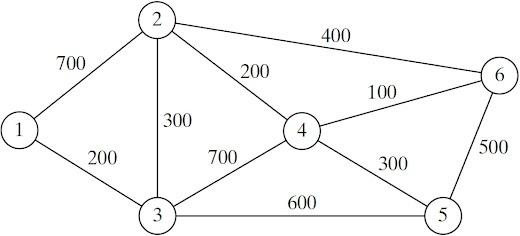
\includegraphics[width=0.4\textwidth]{img/graf-floyd.jpeg}
        \caption{Representacion gráfica de un grafo.}
    \end{figure}

    \begin{figure}[H]
        \centering
         \subfloat[ASUS]{
          \label{asus:floyd-emp}
           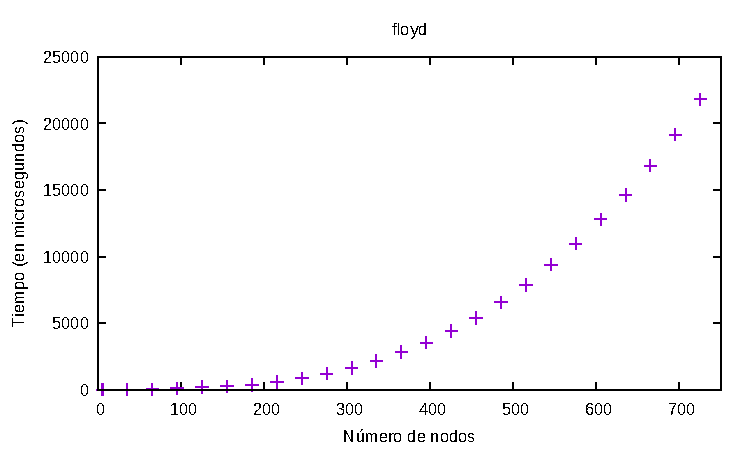
\includegraphics[width=0.7\textwidth]{../data/asus/floyd-points.pdf}}

         \subfloat[HP]{
          \label{hp:floyd-emp}
           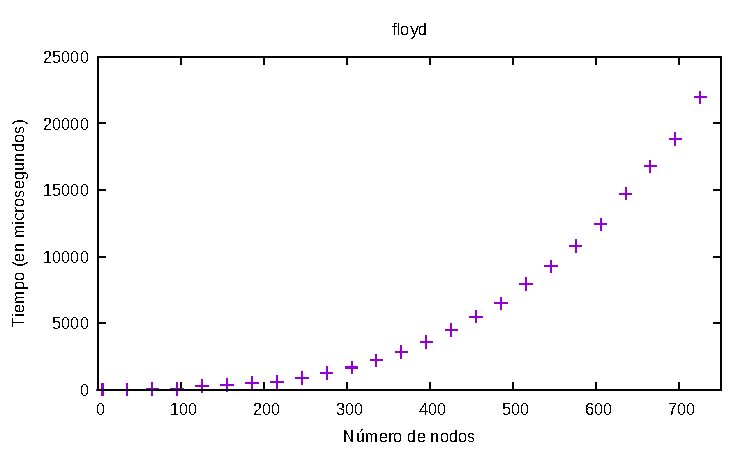
\includegraphics[width=0.7\textwidth]{../data/hp/floyd-points.pdf}}

         \subfloat[LENOVO]{
          \label{lenovo:floyd-emp}
           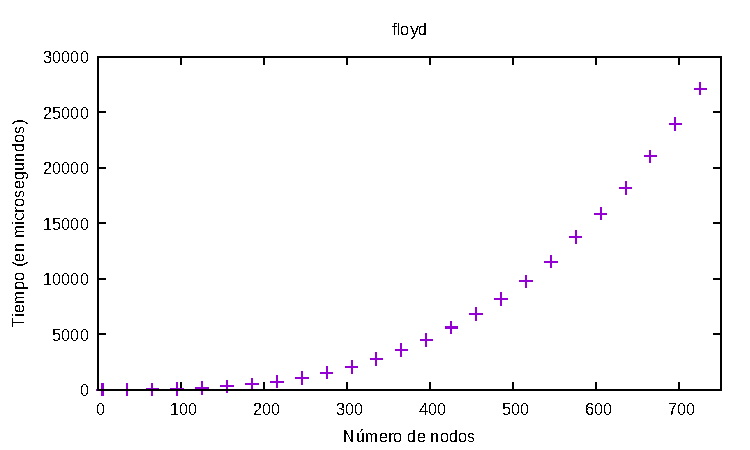
\includegraphics[width=0.7\textwidth]{../data/lenovo/floyd-points.pdf}}
        \caption{Representación gráfica de tiempos de ejecución del algoritmo Floyd.}

        \label{emp:floyd}
    \end{figure}

    \newpage
    
    \subsection{Algoritmo Hanoi}

    En la siguiente tabla se encuentran los datos obtenidos en este algoritmo por cada uno de los
    equipos en los que hemos ejecutado el algoritmo. 

    \begin{table}[h]
        \centering
        \begin{tabular}{|r|r|r|r|}
            \hline
            \text{$N_{disk}$} & \text{$t_{ASUS}$} & \text{$t_{HP}$} & \text{$t_{LENOVO}$} \\
            \hline
            2 & 0.04 & 0.10 & 0.16 \\ 
            3 & 0.08 & 0.10 & 0.20 \\ 
            4 & 0.08 & 0.14 & 0.20 \\ 
            6 & 0.08 & 0.42 & 0.22 \\ 
            7 & 0.24 & 0.36 & 0.26 \\ 
            8 & 0.18 & 0.50 & 0.48 \\ 
            10 & 0.22 & 0.84 & 0.52 \\ 
            11 & 0.36 & 1.22 & 0.74 \\ 
            12 & 1.10 & 3.90 & 1.88 \\ 
            13 & 2.38 & 6.52 & 4.06 \\ 
            14 & 5.26 & 6.26 & 6.98 \\ 
            16 & 10.40 & 11.82 & 14.02 \\ 
            17 & 41.72 & 47.08 & 51.68 \\ 
            18 & 83.38 & 97.78 & 101.66 \\ 
            20 & 170.68 & 313.84 & 199.10 \\ 
            21 & 340.14 & 494.60 & 373.10 \\ 
            22 & 1185.76 & 1084.10 & 1605.38 \\ 
            23 & 1776.36 & 2082.46 & 2712.62 \\ 
            24 & 3295.08 & 3465.74 & 4693.84 \\ 
            26 & 6642.10 & 6844.50 & 9232.04 \\ 
            \hline
        \end{tabular}
        \caption{Tiempos de ejecución (en $\mu$s) del algoritmo de Hanoi}
    \end{table}

    Verificando los resultados obtenidos en los análisis anteriores, para el algoritmo de hanoi, ASUS ofrece unos mejores 
    tiempos de ejecución, seguido de HP y en último lugar LENOVO, que genera tiempos de ejecución mayores. 

    \begin{figure}[h]
        \centering
        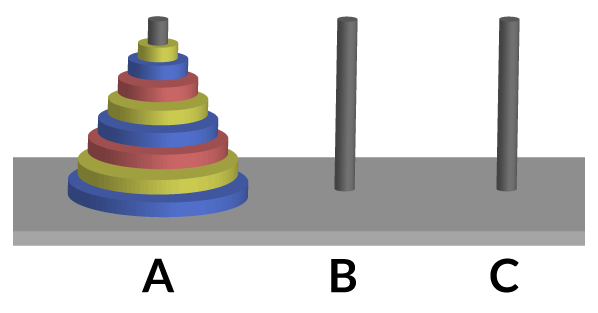
\includegraphics[width=0.4\textwidth]{img/hanoi.png}
        \caption{Representacion gráfica del juego de las Torres de Hanoi.}
    \end{figure}

    Ahora vamos a mostrar las gráficas resultantes tras calcular el tiempo que tarda la ejecución de este algoritmo para diferentes
    tamaños, en este caso, para distinto número de discos.

    \begin{figure}[H]
        \centering
         \subfloat[ASUS]{
          \label{asus:hanoi-emp}
           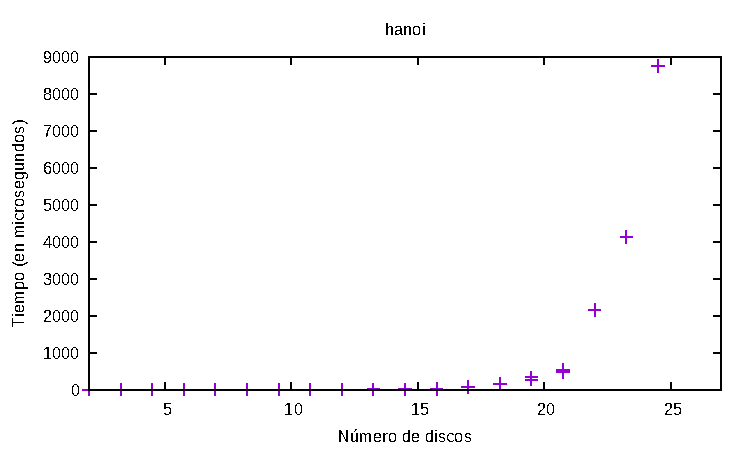
\includegraphics[width=0.7\textwidth]{../data/asus/hanoi-points.pdf}}

         \subfloat[HP]{
          \label{hp:hanoi-emp}
           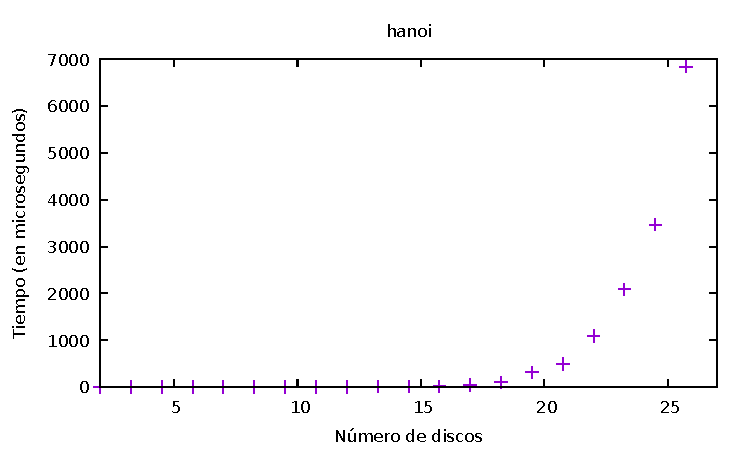
\includegraphics[width=0.7\textwidth]{../data/hp/hanoi-points.pdf}}

         \subfloat[LENOVO]{
          \label{lenovo:hanoi-emp}
           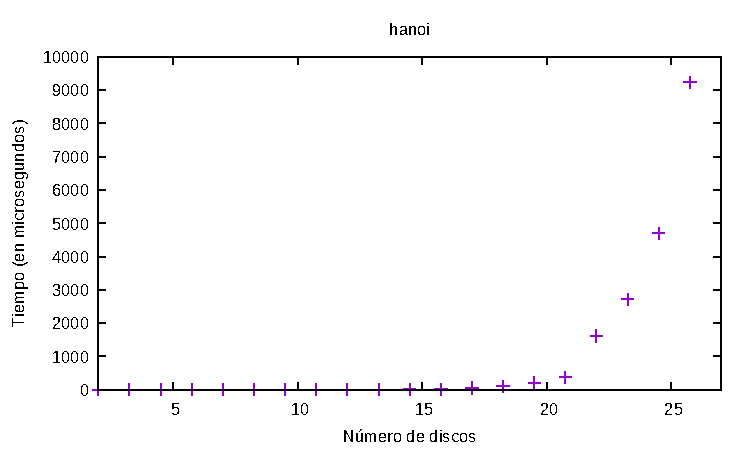
\includegraphics[width=0.7\textwidth]{../data/lenovo/hanoi-points.pdf}}
        \caption{Representación gráfica de tiempos de ejecución del algoritmo de resolución del juego de las Torres de Hanoi.}

        \label{emp:hanoi}
    \end{figure}

    \newpage
    \section{Comparación de ejecuciones con diferentes niveles de optimización}

    \subsection{Conceptos teóricos}

    A continuación, usaremos el algoritmo de Floyd para ilustrar uno de los objetivos mencionados de la práctica, 
    el cual consiste en analizar la eficiencia de un mismo algoritmo para optimizaciones del compilador diferentes.
    En concreto, al igual que en el resto de ejecuciones, usamos g++ como compilador, y analizaremos las siguientes
    opciones de optimización:

    \begin{itemize}
        \item \textbf{-O0 (sin optimización)}: Desconecta por completo la optimización y es el predeterminado si 
        no se especifica ningún nivel.
        \item \textbf{-O1}: El nivel de optimización más básico. El compilador intentará producir un código rápido
        y pequeño sin tomar mucho tiempo de compilación. 
        \item \textbf{-O2}: Un paso delante de -O1. Es el nivel recomendado de optimización, a no ser que el sistema
        tenga necesidades especiales. -O2 activará algunas opciones añadidas a las que se activan con -O1. 
        Con -O2, el compilador intentará aumentar el rendimiento del código sin comprometer el tamaño y sin tomar 
        mucho más tiempo de compilación.
        \item \textbf{-O3}:  El nivel más alto de optimización posible. Activa optimizaciones que son caras en términos 
        de tiempo de compilación y uso de memoria. El hecho de compilar con -O3 no garantiza una forma de mejorar el 
        rendimiento y, de hecho, en muchos casos puede ralentizar un sistema debido al uso de binarios de gran tamaño y 
        mucho uso de la memoria.
    \end{itemize} 
    
    \subsection{Tablas de ejecución} 

    Los tiempos de ejecución para los diferentes niveles de optimización se presentan en la siguiente tabla. 

    \begin{table}[H]
        \centering
        \begin{tabular}{|r|r|r|r|r|}
            \hline
            $N_{nodos}$ & $T_{O0}$ & $T_{O1}$ & $T_{O2}$ & $T_{O3}$ \\
            \hline
            5 & 0.17 & 0.08 & 0.06 & 0.07 \\ 
            35 & 53.95 & 4.47 & 3.02 & 3.52 \\ 
            65 & 380.01 & 27.30 & 26.04 & 35.80 \\ 
            95 & 490.60 & 92.52 & 124.14 & 127.20 \\ 
            125 & 841.45 & 205.10 & 275.73 & 198.03 \\ 
            155 & 1494.98 & 386.86 & 360.05 & 219.22 \\ 
            185 & 2494.07 & 447.26 & 367.53 & 368.06 \\ 
            215 & 3892.51 & 688.94 & 564.97 & 573.63 \\ 
            245 & 5761.86 & 1032.51 & 849.70 & 843.58 \\ 
            275 & 8168.23 & 1443.59 & 1183.75 & 1205.76 \\ 
            305 & 10994.11 & 1997.49 & 1617.42 & 1629.11 \\ 
            335 & 14597.46 & 2648.92 & 2166.47 & 2158.78 \\ 
            365 & 19297.67 & 3386.93 & 2794.19 & 2793.36 \\ 
            395 & 24360.22 & 4255.16 & 3517.28 & 3520.41 \\ 
            425 & 30149.47 & 5370.36 & 4386.85 & 4494.97 \\ 
            455 & 37490.57 & 6552.51 & 5482.11 & 5511.59 \\ 
            485 & 46042.69 & 7993.95 & 6694.07 & 6717.87 \\ 
            515 & 53611.57 & 9620.67 & 7998.24 & 7933.97 \\ 
            545 & 63969.28 & 11346.75 & 9421.14 & 9432.59 \\ 
            575 & 76580.04 & 13442.25 & 11065.08 & 11010.14 \\ 
            605 & 87898.27 & 15581.91 & 12906.25 & 12797.45 \\ 
            635 & 102621.15 & 18516.74 & 14833.09 & 14603.30 \\ 
            665 & 117634.85 & 21025.31 & 16875.94 & 16933.83 \\ 
            695 & 133193.50 & 23857.43 & 19786.48 & 19152.38 \\ 
            725 & 152998.80 & 27005.65 & 22494.99 & 22495.65 \\ 
            \hline
        \end{tabular}
        \caption{Tiempos de ejecución (en $\mu$s) para algoritmo Floyd (Asus)}
    \end{table}

    \begin{figure}[H]
        \centering
        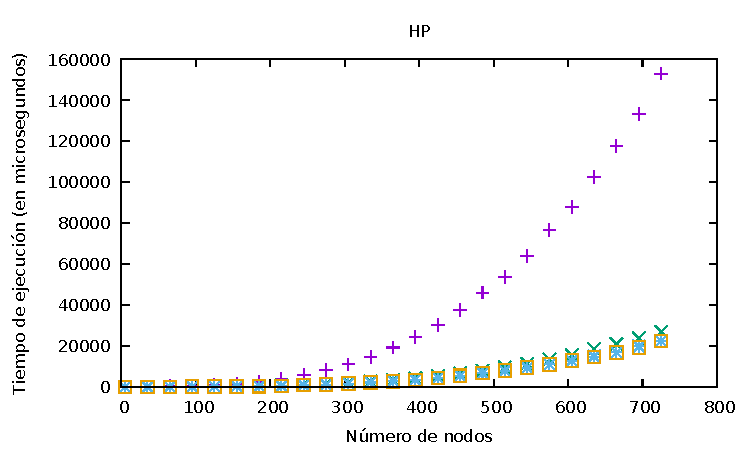
\includegraphics[width=0.6\textwidth]{../data/asus-opt.pdf}
        \caption{Gráfica de tiempos de ejecución (Asus)}
    \end{figure}

    \begin{table}[H]
        \centering
        \begin{tabular}{|r|r|r|r|r|}
            \hline
            $N_{nodos}$ & $T_{O0}$ & $T_{O1}$ & $T_{O2}$ & $T_{O3}$ \\
            \hline
            5 & 0.21 & 0.10 & 0.09 & 0.10 \\ 
            35 & 39.48 & 3.78 & 6.07 & 5.20 \\ 
            65 & 251.96 & 46.40 & 48.65 & 42.72 \\ 
            95 & 574.10 & 179.56 & 146.43 & 145.99 \\ 
            125 & 793.83 & 301.52 & 266.95 & 175.65 \\ 
            155 & 1510.12 & 286.76 & 318.89 & 309.46 \\ 
            185 & 2495.91 & 449.75 & 376.88 & 404.58 \\ 
            215 & 3914.89 & 708.44 & 577.90 & 586.26 \\ 
            245 & 5701.98 & 1028.52 & 853.82 & 875.53 \\ 
            275 & 8082.82 & 1492.51 & 1207.13 & 1231.23 \\ 
            305 & 10928.36 & 1971.31 & 1638.46 & 1670.67 \\ 
            335 & 14455.55 & 2698.91 & 2178.86 & 2174.05 \\ 
            365 & 18929.88 & 3473.24 & 2837.69 & 2833.66 \\ 
            395 & 24332.74 & 4414.80 & 3564.82 & 3646.11 \\ 
            425 & 29848.49 & 5443.34 & 4421.02 & 4510.19 \\ 
            455 & 36908.89 & 6591.26 & 5360.57 & 5432.05 \\ 
            485 & 44582.97 & 8053.35 & 6493.54 & 6667.46 \\ 
            515 & 53470.68 & 9527.39 & 7778.40 & 7889.72 \\ 
            545 & 63172.00 & 11443.67 & 9345.16 & 9462.12 \\ 
            575 & 75819.62 & 13436.56 & 10767.32 & 10656.11 \\ 
            605 & 86390.05 & 15466.07 & 12933.42 & 12717.99 \\ 
            635 & 100187.65 & 17941.33 & 14708.66 & 14143.55 \\ 
            665 & 117042.70 & 20676.88 & 16400.16 & 16729.92 \\ 
            695 & 131518.20 & 23515.96 & 18637.03 & 19198.70 \\ 
            725 & 147998.15 & 26638.71 & 21326.99 & 21331.96 \\ 
            \hline
        \end{tabular}
        \caption{Tiempos de ejecución (en $\mu$s) para algoritmo Floyd (HP)}
    \end{table}

    \begin{figure}[H]
        \centering
        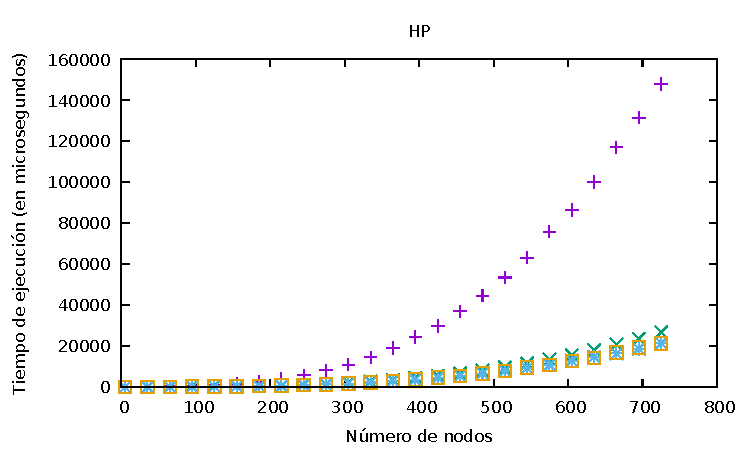
\includegraphics[width=0.6\textwidth]{../data/hp_opt.pdf}
        \caption{Gráfica de tiempos de ejecución (HP)}
    \end{figure}


    \begin{table}[H]
        \centering
        \begin{tabular}{|r|r|r|r|r|}
            \hline
            $N_{nodos}$ & $T_{O0}$ & $T_{O1}$ & $T_{O2}$ & $T_{O3}$ \\
            \hline
            5 & 0.23 & 0.17 & 0.23 & 0.33 \\ 
            35 & 29.84 & 6.48 & 5.50 & 5.55 \\ 
            65 & 203.45 & 35.44 & 31.70 & 37.05 \\ 
            95 & 645.68 & 135.50 & 126.25 & 116.51 \\ 
            125 & 1138.86 & 294.69 & 266.38 & 199.54 \\ 
            155 & 2220.49 & 530.83 & 466.20 & 370.52 \\ 
            185 & 3524.26 & 866.54 & 794.60 & 661.22 \\ 
            215 & 5531.06 & 1340.55 & 1108.49 & 1120.88 \\ 
            245 & 9879.07 & 2039.46 & 1490.56 & 1765.31 \\ 
            275 & 14760.01 & 2775.61 & 1988.81 & 2839.12 \\ 
            305 & 21002.12 & 3709.97 & 2736.05 & 2645.93 \\ 
            335 & 21130.67 & 4774.23 & 3574.84 & 4324.62 \\ 
            365 & 28563.90 & 5061.25 & 4065.97 & 4587.72 \\ 
            395 & 35266.89 & 7312.15 & 5092.35 & 6049.83 \\ 
            425 & 43856.27 & 9466.16 & 6145.76 & 7357.14 \\ 
            455 & 63704.19 & 11719.27 & 8768.52 & 9735.48 \\ 
            485 & 71028.24 & 15156.26 & 10372.40 & 9273.38 \\ 
            515 & 85424.65 & 24115.51 & 13265.73 & 11000.40 \\ 
            545 & 103213.98 & 16958.10 & 14592.08 & 12854.59 \\ 
            575 & 123200.59 & 18765.49 & 15596.62 & 24142.65 \\ 
            605 & 134205.15 & 20772.30 & 17569.12 & 29495.03 \\ 
            635 & 197191.95 & 31057.76 & 20804.73 & 34560.04 \\ 
            665 & 224866.25 & 27874.88 & 28951.74 & 32018.41 \\ 
            695 & 203138.40 & 35154.18 & 46677.95 & 27752.09 \\ 
            725 & 214510.65 & 50098.56 & 40081.61 & 35497.00 \\ 
            \hline
        \end{tabular}
        \caption{Tiempos de ejecución (en $\mu$s) para algoritmo Floyd (Lenovo)}
    \end{table}

    \begin{figure}[H]
        \centering
        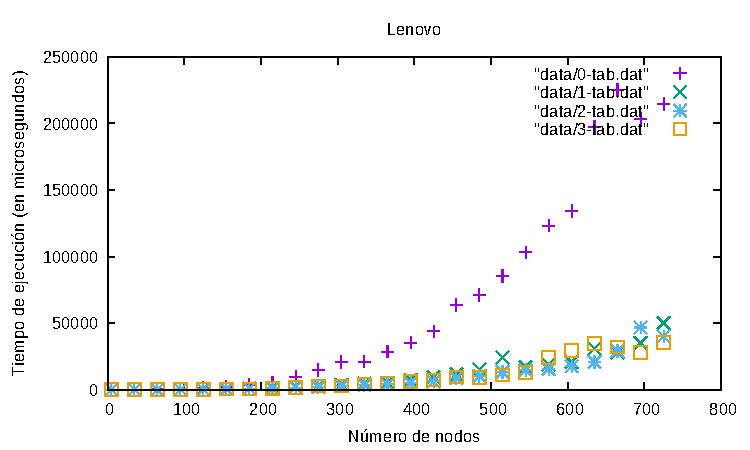
\includegraphics[width=0.6\textwidth]{../data/lenovo-opt.pdf}
        \caption{Gráfica de tiempos de ejecución (Lenovo)}
    \end{figure}

    \vspace{3cm} 

    \subsection{Observaciones}

    Observando las gráficas se puede apreciar que, para pequeños valores del número de nodos, las diferencias entre los
    tiempos de ejecución para diferentes niveles de optimización son prácticamente despreciables. Sin embargo, a medida
    que va aumentando la complejidad del grafo, los tiempos de ejecución para diferentes niveles de optimización se hacen
    más significativos, siendo que para $n \geq 300$, se empieza a hacer palpable dicha mejoría. 

    Por tanto, concluimos que, para ejecuciones de tamaños pequeños, las diferencias son apenas apreciables, mientras que
    para grandes valores la optimización sí que puede aumentar considerablemente los tiempos de ejecución. Se trata, por
    consiguiente, de un buen mecanismo de optimización del código. 

    \newpage
    \section{Comparación de los algoritmos de ordenación}

    \subsection{Objetivos}

    En esta sección compararemos los algoritmos de ordenación presentados previamente. El objetivo será
    sacar conclusiones relevantes relacionados con la adecuación de cada algoritmo a cada situación. Los datos de ejecución
    se presentan a continuación:

    \begin{table}[H]
        \footnotesize
        \centering
        \begin{tabular}{|r|r|r|r|r|}
            \hline
            $N_{componentes}$ & $T_{\text{quick}}$ & $T_{\text{heap}}$ & $T_{\text{ins}}$ & $T_{\text{sel}}$ \\
            \hline
            50 & 0.17 & 0.23 & 0.20 & 0.00 \\ 
            1550 & 6.61 & 9.05 & 75.77 & 0.00 \\ 
            3050 & 14.03 & 18.94 & 256.80 & 405.64 \\ 
            4550 & 22.15 & 29.91 & 568.78 & 887.38 \\ 
            6050 & 30.74 & 41.86 & 1009.34 & 1743.89 \\ 
            7550 & 39.04 & 48.98 & 1563.83 & 2516.84 \\ 
            9050 & 46.95 & 59.41 & 2223.38 & 3478.01 \\ 
            10550 & 56.34 & 73.60 & 3041.16 & 4687.76 \\ 
            12050 & 71.14 & 111.73 & 3990.62 & 6069.77 \\ 
            13550 & 89.81 & 134.07 & 5006.11 & 7622.48 \\ 
            15050 & 88.45 & 91.58 & 6150.48 & 9379.73 \\ 
            16550 & 98.56 & 100.37 & 7465.37 & 11353.25 \\ 
            18050 & 107.69 & 110.64 & 8826.78 & 13419.11 \\ 
            19550 & 117.73 & 120.14 & 10378.18 & 15720.16 \\ 
            21050 & 127.28 & 130.39 & 11990.83 & 18222.62 \\ 
            22550 & 117.67 & 229.32 & 13870.88 & 20890.26 \\ 
            24050 & 115.74 & 175.66 & 15767.71 & 23723.39 \\ 
            25550 & 129.62 & 182.04 & 17623.01 & 26674.83 \\ 
            27050 & 130.34 & 171.59 & 19843.40 & 29887.24 \\ 
            28550 & 137.97 & 182.18 & 22034.17 & 33262.06 \\ 
            30050 & 147.05 & 193.19 & 24340.38 & 36738.72 \\ 
            31550 & 191.97 & 203.78 & 27098.83 & 40416.56 \\ 
            33050 & 191.03 & 214.28 & 29862.88 & 44399.06 \\ 
            34550 & 192.52 & 226.52 & 32503.73 & 48514.63 \\ 
            36050 & 197.37 & 234.89 & 35181.93 & 52767.88 \\ 
            37550 & 210.15 & 246.49 & 38327.38 & 57179.00 \\ 
            39050 & 219.80 & 256.88 & 41369.21 & 61972.05 \\ 
            40550 & 231.73 & 268.05 & 44358.82 & 66553.92 \\ 
            42050 & 238.25 & 278.93 & 48124.07 & 71651.73 \\ 
            43550 & 262.80 & 290.42 & 51624.04 & 76278.35 \\ 
            \hline
        \end{tabular}
        \caption{Tabla de comparación de tiempos de ejecución entre algoritmos de ordenación (Asus)}
    \end{table}

    \begin{figure}[H]
        \centering
        \label{asus:orden}
        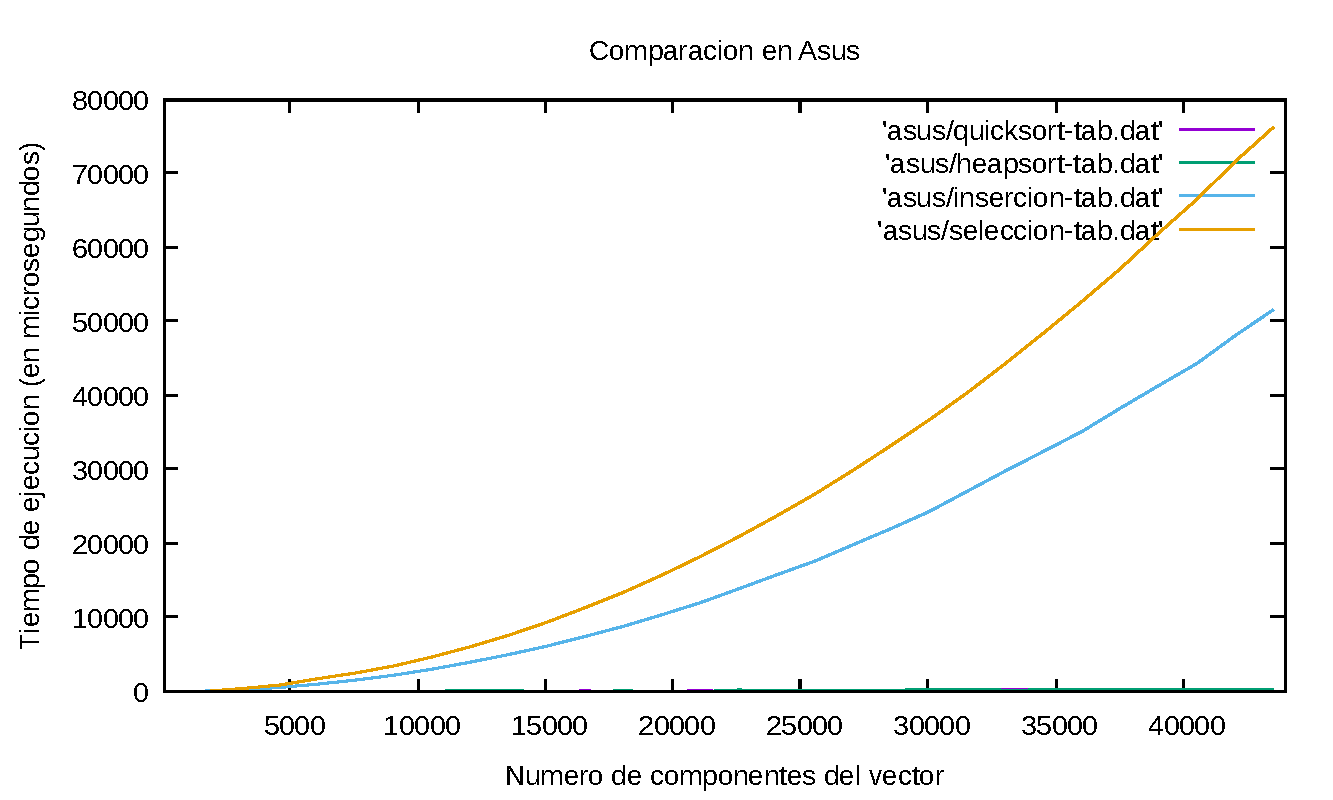
\includegraphics[width=0.5\textwidth]{../data/asus-orden-todos.pdf}
        \caption{Gráfico de comparación de algoritmos de ordenación (ASUS)}
    \end{figure}

    \begin{table}[H]
        \footnotesize
        \centering
        \begin{tabular}{|r|r|r|r|r|}
            \hline
            $N_{componentes}$ & $T_{\text{quick}}$ & $T_{\text{heap}}$ & $T_{\text{ins}}$ & $T_{\text{sel}}$ \\
            \hline
            50 & 0.52 & 0.22 & 0.18 & 0.26 \\ 
            1550 & 6.61 & 7.20 & 65.22 & 93.16 \\ 
            3050 & 12.35 & 15.26 & 321.24 & 365.10 \\ 
            4550 & 17.27 & 26.14 & 647.40 & 940.48 \\ 
            6050 & 23.82 & 48.90 & 1036.40 & 1488.90 \\ 
            7550 & 34.79 & 71.06 & 1618.74 & 2126.38 \\ 
            9050 & 36.57 & 110.92 & 2280.68 & 3021.74 \\ 
            10550 & 40.18 & 153.54 & 3017.28 & 4092.94 \\ 
            12050 & 50.55 & 177.70 & 4005.42 & 5308.02 \\ 
            13550 & 55.28 & 204.18 & 5016.44 & 6881.72 \\ 
            15050 & 61.57 & 228.52 & 6221.24 & 8541.68 \\ 
            16550 & 70.63 & 251.66 & 7543.96 & 10907.70 \\ 
            18050 & 75.28 & 277.96 & 8895.32 & 12371.38 \\ 
            19550 & 80.04 & 304.58 & 10479.46 & 13904.10 \\ 
            21050 & 85.59 & 331.72 & 12000.74 & 16005.40 \\ 
            22550 & 90.47 & 355.20 & 13841.24 & 19573.20 \\ 
            24050 & 100.66 & 533.96 & 15701.64 & 20729.80 \\ 
            25550 & 110.87 & 256.20 & 17659.94 & 23292.68 \\ 
            27050 & 117.50 & 190.04 & 19860.74 & 28970.88 \\ 
            28550 & 123.90 & 201.76 & 22197.46 & 30344.76 \\ 
            30050 & 131.77 & 212.80 & 24393.30 & 34703.62 \\ 
            31550 & 137.76 & 229.00 & 27505.86 & 37670.52 \\ 
            33050 & 142.09 & 352.70 & 30478.94 & 38029.22 \\ 
            34550 & 153.92 & 404.38 & 33168.82 & 41404.42 \\ 
            36050 & 160.30 & 405.24 & 35869.34 & 44965.98 \\ 
            37550 & 167.35 & 294.02 & 39764.76 & 48548.56 \\ 
            39050 & 170.98 & 306.16 & 42636.54 & 52687.52 \\ 
            40550 & 180.96 & 320.70 & 46448.22 & 56478.82 \\ 
            42050 & 188.74 & 383.94 & 50855.00 & 60501.86 \\ 
            43550 & 200.55 & 331.54 & 54694.44 & 68268.24 \\ 
            \hline
        \end{tabular}
        \caption{Tabla de comparación de tiempos de ejecución entre algoritmos de ordenación (HP)}
    \end{table}

    \begin{figure}[H]
        \centering
        \label{hp:orden}
        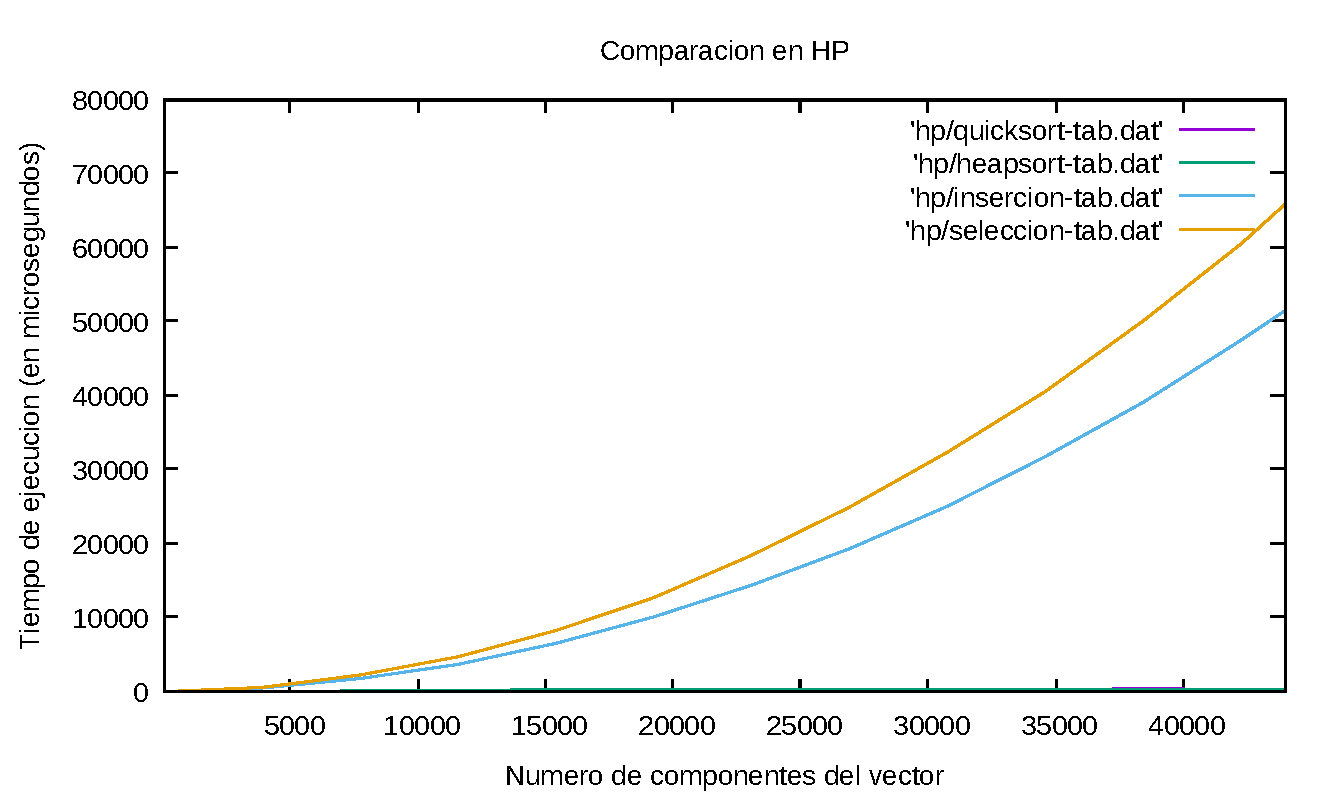
\includegraphics[width=0.7\textwidth]{../data/hp_orden-todos.pdf}
        \caption{Gráfico de comparación de algoritmos de ordenación (HP)}
    \end{figure}

    \begin{table}[H]
        \footnotesize
        \centering
        \begin{tabular}{|r|r|r|r|r|}
            \hline
            $N_{componentes}$ & $T_{\text{quick}}$ & $T_{\text{heap}}$ & $T_{\text{ins}}$ & $T_{\text{sel}}$ \\
            \hline
            50 & 0.35 & 0.58 & 0.32 & 0.34 \\ 
            1550 & 15.56 & 30.47 & 113.40 & 150.44 \\ 
            3050 & 39.12 & 48.51 & 416.61 & 517.39 \\ 
            4550 & 39.49 & 60.96 & 818.87 & 1151.71 \\ 
            6050 & 61.13 & 67.12 & 1318.29 & 1969.91 \\ 
            7550 & 64.00 & 76.26 & 2040.42 & 3044.82 \\ 
            9050 & 67.17 & 105.57 & 2893.16 & 4373.70 \\ 
            10550 & 77.66 & 118.94 & 3937.94 & 5785.53 \\ 
            12050 & 90.32 & 138.07 & 5111.43 & 8933.87 \\ 
            13550 & 101.90 & 163.47 & 6412.50 & 13236.58 \\ 
            15050 & 119.67 & 176.82 & 7911.75 & 16256.42 \\ 
            16550 & 134.65 & 180.48 & 9605.05 & 19545.66 \\ 
            18050 & 145.62 & 209.31 & 11396.08 & 23262.00 \\ 
            19550 & 150.02 & 221.17 & 13402.47 & 27114.96 \\ 
            21050 & 163.49 & 231.88 & 15511.25 & 31358.34 \\ 
            22550 & 175.83 & 259.55 & 17763.31 & 35875.34 \\ 
            24050 & 187.89 & 266.38 & 20213.18 & 41767.30 \\ 
            25550 & 205.24 & 283.95 & 22797.11 & 50257.00 \\ 
            27050 & 214.19 & 312.24 & 25575.44 & 57776.30 \\ 
            28550 & 228.24 & 322.75 & 28426.29 & 62347.18 \\ 
            30050 & 245.48 & 342.44 & 31521.96 & 63689.96 \\ 
            31550 & 254.54 & 368.07 & 34782.56 & 70027.92 \\ 
            33050 & 269.09 & 388.03 & 38191.71 & 83165.06 \\ 
            34550 & 281.52 & 405.24 & 41713.63 & 91810.12 \\ 
            36050 & 299.20 & 428.18 & 45353.92 & 78691.24 \\ 
            37550 & 326.10 & 446.28 & 49245.56 & 76481.60 \\ 
            39050 & 329.71 & 456.01 & 53230.43 & 81182.66 \\ 
            40550 & 336.20 & 481.33 & 57379.06 & 90248.08 \\ 
            42050 & 346.37 & 504.41 & 61712.14 & 93852.48 \\ 
            43550 & 358.76 & 518.26 & 66215.14 & 103615.64 \\ 
            \hline
        \end{tabular}
        \caption{Tabla de comparación de tiempos de ejecución entre algoritmos de ordenación (Lenovo)}

    \end{table}

    \begin{figure}[H]
        \centering
        \label{lenovo:orden}
           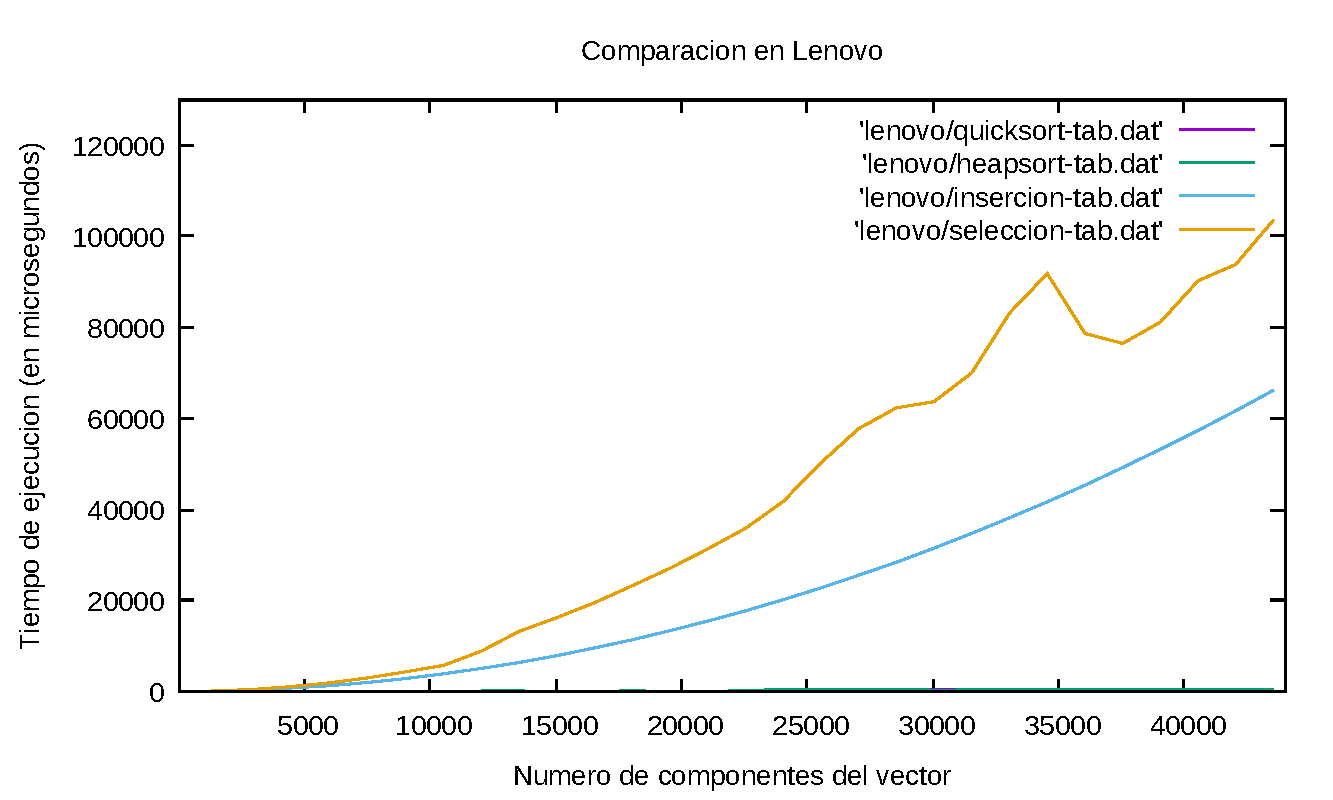
\includegraphics[width=0.7\textwidth]{../data/lenovo-orden-todos.pdf}
        \caption{Gráfico de comparación de algoritmos de ordenación (Lenovo)}
    \end{figure}

    \vspace{2cm}

    \subsection{Conclusiones}
    
    De las gráficas extraídas anteriores, podemos sacar las siguientes conclusiones:
    
    \begin{itemize}
        \item Para grandes valores de componentes de vector, los algoritmos de HeapSort y QuickSort presentan un muy buen comportamiento.
        \item Los algoritmos de inserción y de selección ofrecen peor rendimiento respecto a QuickSort y HeapSort (su orden de eficiencia es mayor).
        \item Para tamaños pequeños, las diferencias entre los cuatro algoritmos son prácticamente despreciables, por lo que su uso debería optarse más por la facilidad de implementación de dichos algoritmos. 
        \item El mínimo valor $n_0$ a partir del cual el tiempo de ejecución de los algoritmos de Inserción y de Selección superan a los de QuickSort y HeapSort es tan pequeño que es despreciable. 
              La mejor cota que tenemos, teniendo en cuenta los datos obtenidos, es que $n_0 \leq 5$. 
    \end{itemize}

    \newpage
    \section{Eficiencia de mejor y peor caso en los algoritmos de Inserción y Selección}

    El número de operaciones elementales que se realizan en cada uno de los algoritmos que hemos analizado fluctúan 
    en gran medida en función de la configuración inicial de los valores de entrada. En esta sección analizaremos los
    algoritmos de Inserción y de Selección tanto para el mejor como el peor caso.

    \subsection{Fundamento teórico}

    Para ambos algoritmos, cuando nos fijamos en sus implementaciones podemos observar que el mayor número de operaciones
    elementales se realizan cuando los vectores están ordenados en orden decreciente (esto es, $a_n > a_{n+1}$, $\forall n \in \mathbb N$).
    Asimismo, cuando los vectores están totalmente ordenados en orden creciente, el número de operaciones es mínima ($a_n < a_{n+1}$, $\forall n \in \mathbb N$).

    Por tanto, para poder probar tanto los mejores casos como los peores casos, se han creado 4 nuevos archivos fuentes, donde
    2 proceden del mejor y peor caso para Inserción y 2 proceden del análogo para Selección. El único cambio con respecto a los originales es que,
    en lugar de inicializar los vectores con valores aleatorios, se ha optado por inicializar los valores con un cierto orden.

    \subsection{Resultados para Selección}

    Realizando lo expuesto en la subsección anterior, obtenemos las siguientes tablas y gráficas:

    \begin{table}[H] 
        \footnotesize
        \centering 
        \begin{tabular}{|r|r|r|r|} 
                \hline
                $N_{\text{componentes}}$ & $T_{\text{mejor}}$ & $T_{\text{prom}}$ & $T_{\text{peor}}$ \\
                \hline 
                5 & 0.00 & 0.00 & 0.00 \\ 
                1807 & 79.25 & 0.00 & 98.34 \\ 
                3609 & 302.46 & 405.64 & 384.96 \\ 
                5410 & 675.37 & 887.38 & 859.75 \\ 
                7212 & 1200.41 & 1743.89 & 1557.07 \\ 
                9014 & 1865.43 & 2516.84 & 2434.85 \\ 
                10816 & 2680.60 & 3478.01 & 3537.88 \\ 
                12618 & 3647.47 & 4687.76 & 4825.15 \\ 
                14419 & 4768.91 & 6069.77 & 6297.90 \\ 
                16221 & 6045.11 & 7622.48 & 8010.68 \\ 
                18023 & 7531.93 & 9379.73 & 9880.52 \\ 
                19825 & 9108.94 & 11353.25 & 11988.52 \\ 
                21627 & 10741.06 & 13419.11 & 14093.90 \\ 
                23428 & 12711.52 & 15720.16 & 16495.94 \\ 
                25230 & 14687.18 & 18222.62 & 19253.56 \\ 
                27032 & 16892.80 & 20890.26 & 21942.20 \\ 
                28834 & 19175.36 & 23723.39 & 25006.22 \\ 
                30636 & 21719.94 & 26674.83 & 28337.50 \\ 
                32437 & 24472.16 & 29887.24 & 31665.06 \\ 
                34239 & 27386.98 & 33262.06 & 35232.64 \\ 
                36041 & 30492.62 & 36738.72 & 39015.58 \\ 
                37843 & 33498.48 & 40416.56 & 43223.80 \\ 
                39645 & 36693.26 & 44399.06 & 46602.86 \\ 
                41446 & 40339.20 & 48514.63 & 52053.40 \\ 
                43248 & 43518.48 & 52767.88 & 56047.84 \\ 
                \hline
        \end{tabular}
        \caption{Tiempos de ejecución, en $\mu$s, para mejor caso, caso promedio y peor caso (Asus) para Selección}
    \end{table}

    \begin{table}[H]  
        \footnotesize
        \centering 
        \begin{tabular}{|r|r|r|r|} 
                \hline
                $N_{\text{componentes}}$ & $T_{\text{mejor}}$ & $T_{\text{prom}}$ & $T_{\text{peor}}$ \\
                \hline 
                5 & 0.00 & 0.27 & 0.00 \\ 
                1807 & 81.88 & 185.57 & 98.44 \\ 
                3609 & 299.37 & 405.56 & 382.95 \\ 
                5410 & 666.19 & 759.16 & 833.96 \\ 
                7212 & 1180.31 & 1299.40 & 1560.20 \\ 
                9014 & 1838.74 & 2023.15 & 2366.31 \\ 
                10816 & 2633.29 & 2888.28 & 3409.86 \\ 
                12618 & 3621.99 & 3895.39 & 4683.23 \\ 
                14419 & 4697.33 & 5041.98 & 6225.67 \\ 
                16221 & 5960.55 & 6419.54 & 7742.75 \\ 
                18023 & 7381.49 & 7817.24 & 9606.92 \\ 
                19825 & 8863.69 & 9484.57 & 11652.02 \\ 
                21627 & 10595.90 & 11190.25 & 13908.20 \\ 
                23428 & 12586.80 & 13528.89 & 16252.36 \\ 
                25230 & 14547.82 & 15233.13 & 18808.90 \\ 
                27032 & 16827.08 & 17896.47 & 21556.08 \\ 
                28834 & 18727.16 & 20459.99 & 24526.54 \\ 
                30636 & 21006.00 & 22972.99 & 27535.92 \\ 
                32437 & 24335.62 & 25952.09 & 31420.60 \\ 
                34239 & 26681.66 & 28747.80 & 34310.92 \\ 
                36041 & 29371.66 & 32063.87 & 38313.74 \\ 
                37843 & 32222.40 & 35024.40 & 42054.72 \\ 
                39645 & 36061.04 & 38526.17 & 46150.84 \\ 
                41446 & 38442.32 & 40342.34 & 50428.50 \\ 
                43248 & 42317.56 & 43836.76 & 54598.72 \\ 
                \hline
        \end{tabular}
        \caption{Tiempos de ejecución, en $\mu$s, para mejor caso, caso promedio y peor caso (HP) para Selección}
    \end{table}
    
    \begin{table}[H] 
        \footnotesize
        \centering 
        \begin{tabular}{|r|r|r|r|} 
                \hline
                $N_{\text{componentes}}$ & $T_{\text{mejor}}$ & $T_{\text{prom}}$ & $T_{\text{peor}}$ \\
                \hline 
                5 & 0.01 & 0.34 & 0.01 \\ 
                1807 & 103.81 & 150.44 & 171.49 \\ 
                3609 & 400.53 & 517.39 & 614.91 \\ 
                5410 & 901.48 & 1151.71 & 1285.29 \\ 
                7212 & 1585.44 & 1969.91 & 2257.48 \\ 
                9014 & 2439.11 & 3044.82 & 3508.66 \\ 
                10816 & 3507.38 & 4373.70 & 5469.91 \\ 
                12618 & 6351.07 & 5785.53 & 6511.67 \\ 
                14419 & 9539.37 & 8933.87 & 8316.04 \\ 
                16221 & 12871.88 & 13236.58 & 10245.76 \\ 
                18023 & 16066.20 & 16256.42 & 14119.60 \\ 
                19825 & 16408.68 & 19545.66 & 17634.96 \\ 
                21627 & 15898.44 & 23262.00 & 19388.48 \\ 
                23428 & 17792.22 & 27114.96 & 22325.86 \\ 
                25230 & 22375.98 & 31358.34 & 24608.56 \\ 
                27032 & 27522.92 & 35875.34 & 29260.34 \\ 
                28834 & 28345.80 & 41767.30 & 36356.38 \\ 
                30636 & 34513.84 & 50257.00 & 42236.38 \\ 
                32437 & 38301.70 & 57776.30 & 40649.10 \\ 
                34239 & 39776.68 & 62347.18 & 43645.96 \\ 
                36041 & 40343.58 & 63689.96 & 48861.26 \\ 
                37843 & 49479.62 & 70027.92 & 53424.64 \\ 
                39645 & 50629.40 & 83165.06 & 59130.00 \\ 
                41446 & 56755.30 & 91810.12 & 67432.92 \\ 
                43248 & 61439.84 & 78691.24 & 79293.06 \\ 
                \hline
        \end{tabular}
        \caption{Tiempos de ejecución, en $\mu$s, para mejor caso, caso promedio y peor caso (Lenovo) para Selección}
    \end{table}

    \begin{figure}[H]
        \centering
         \subfloat[ASUS]{
          \label{asus:seleccion-mp}
           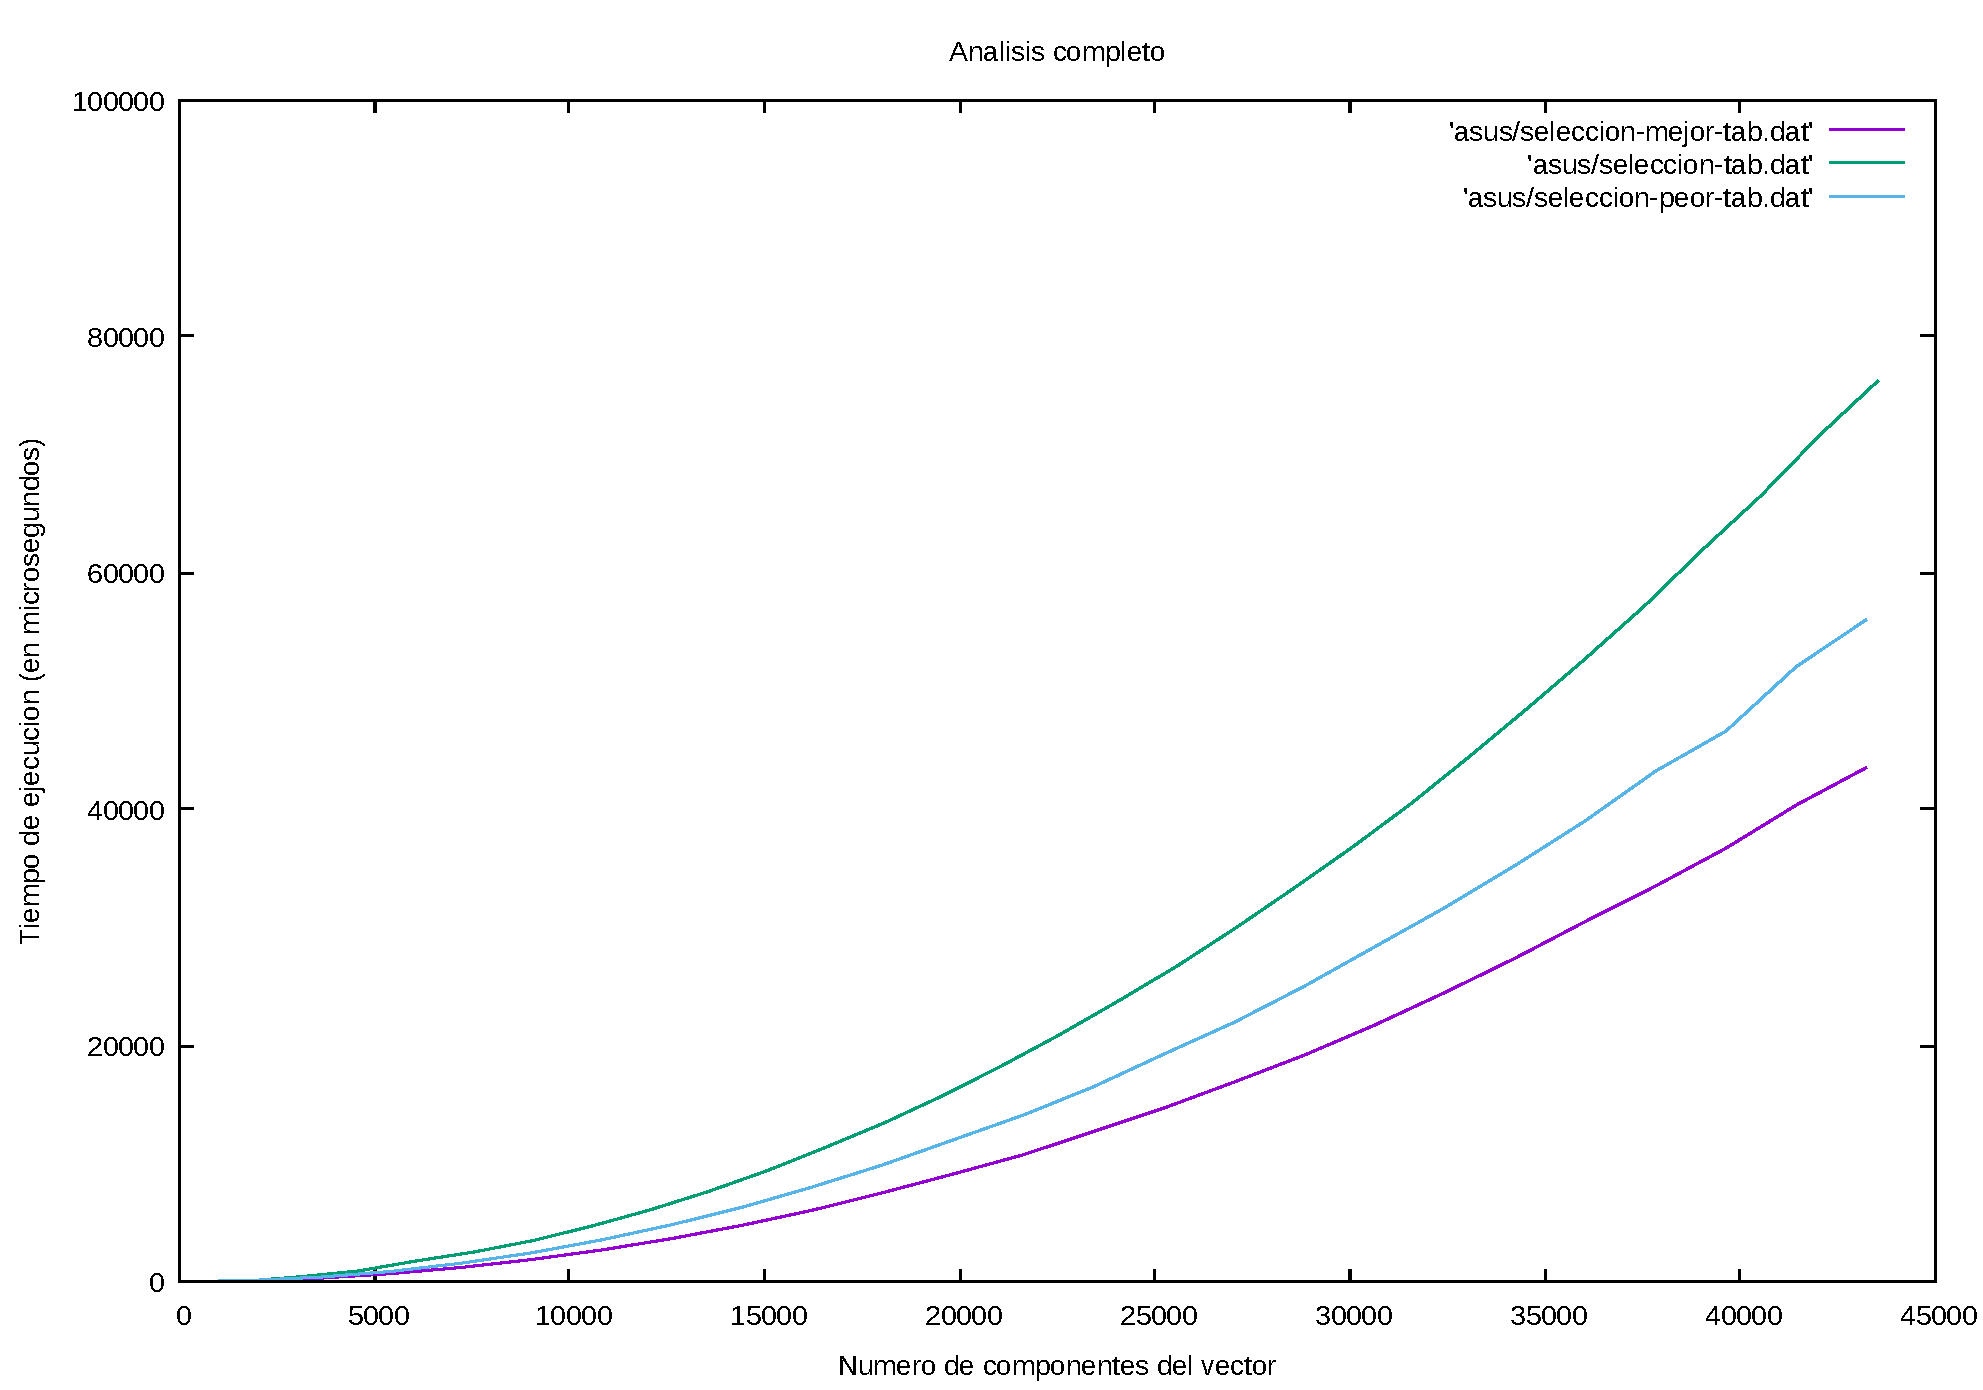
\includegraphics[width=0.63\textwidth]{../data/asus-seleccion-mp.pdf}}

         \subfloat[HP]{
          \label{hp:seleccion-mp}
           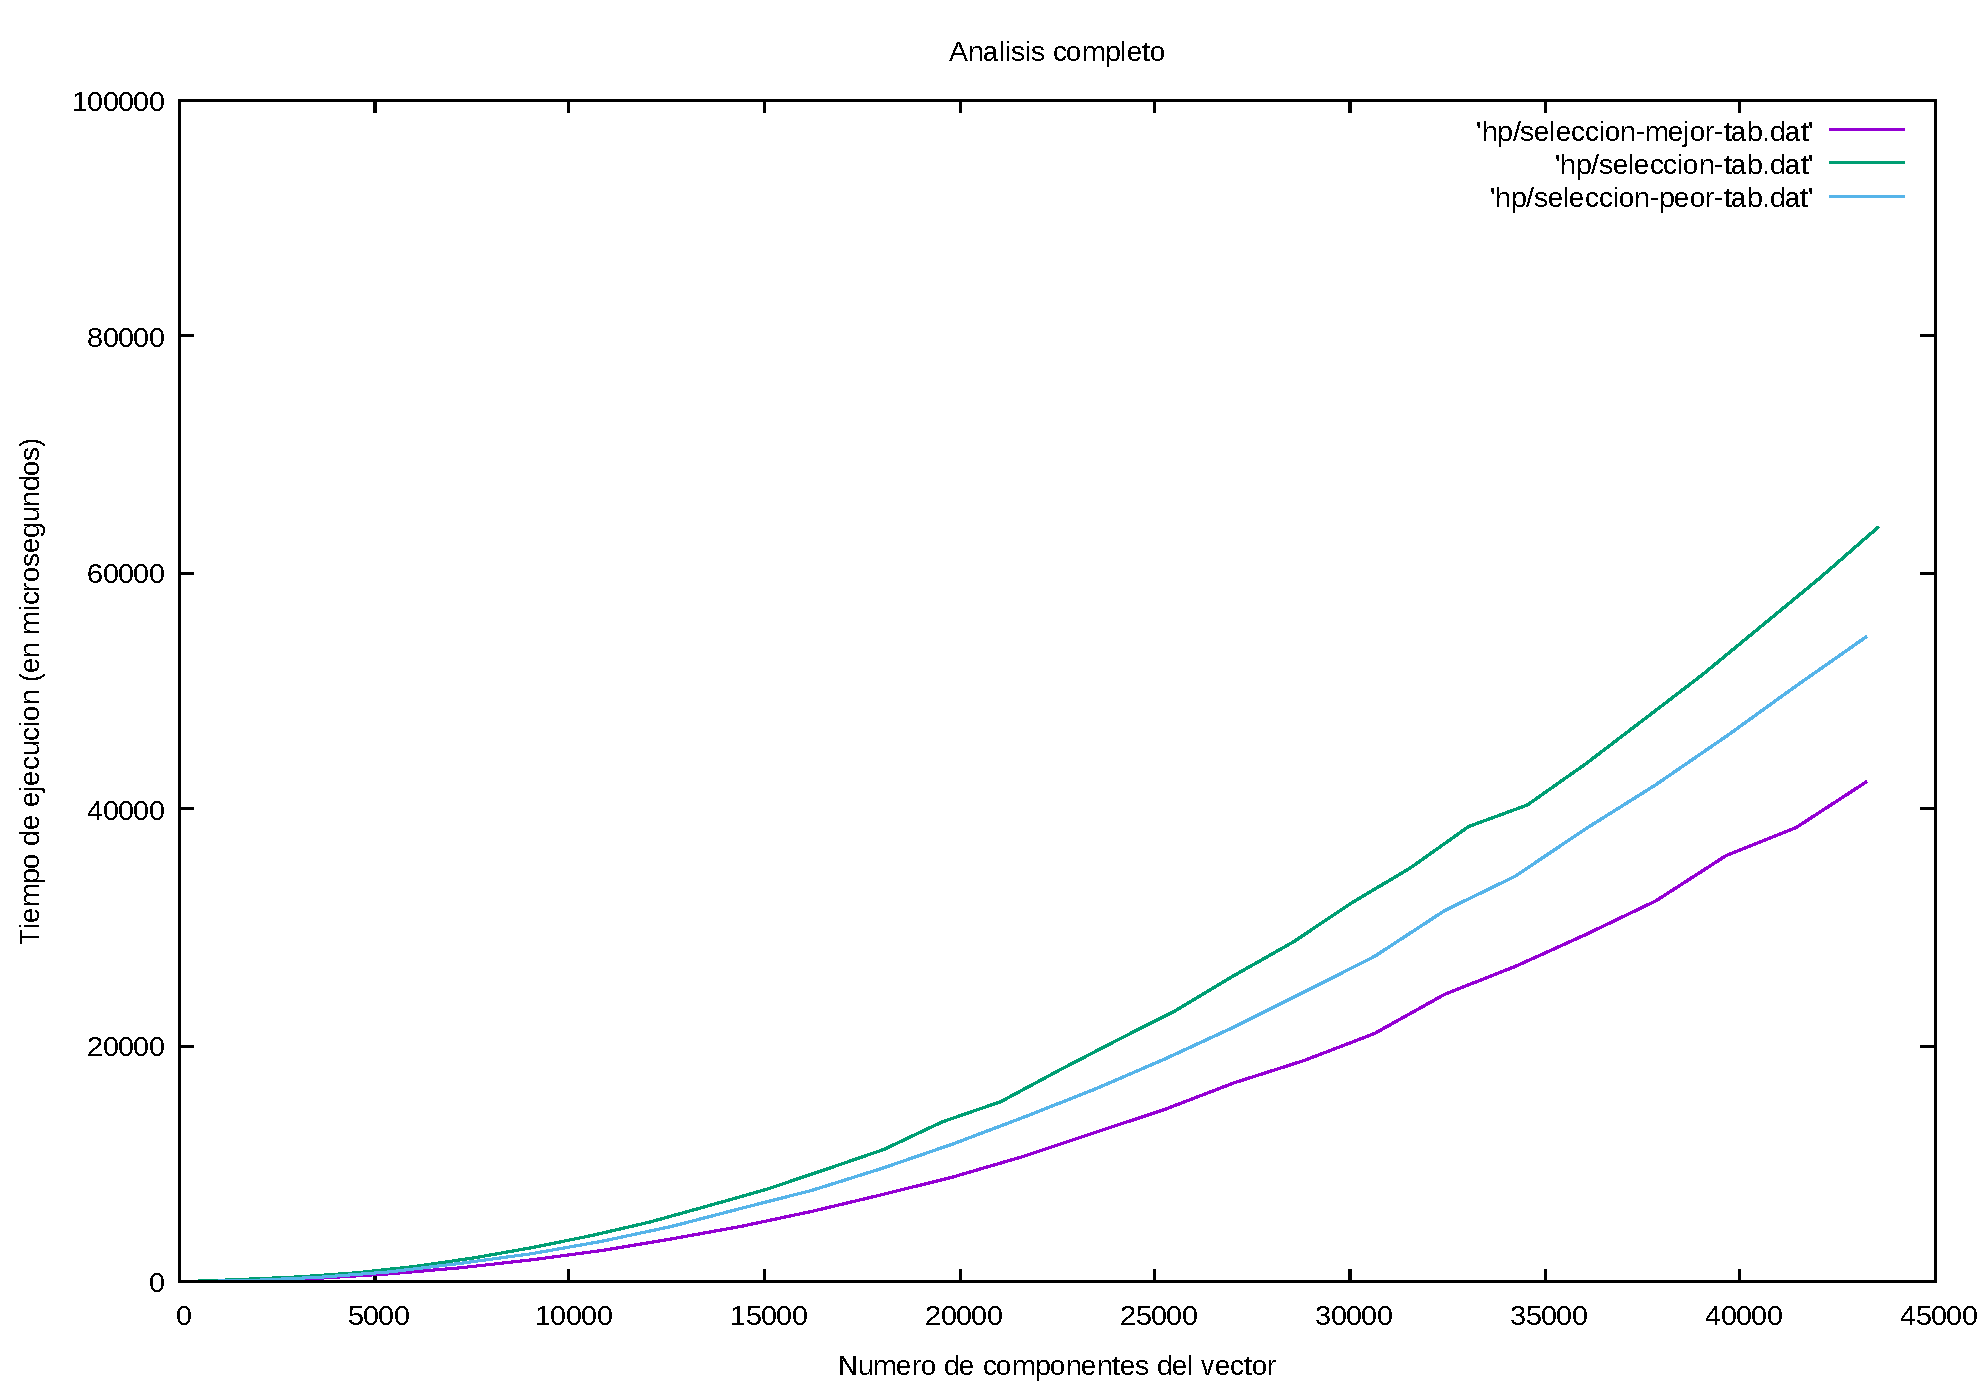
\includegraphics[width=0.63\textwidth]{../data/hp-seleccion-mp.pdf}}

         \subfloat[LENOVO]{
          \label{lenovo:seleccion-mp}
           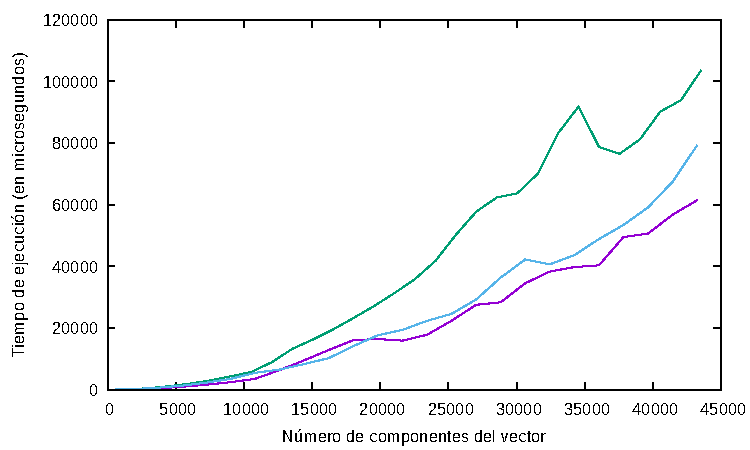
\includegraphics[width=0.63\textwidth]{../data/lenovo-seleccion-mp.pdf}}
        \caption{Gráficas de regresión de los algoritmos de Selección para caso peor, mejor y promedio.}

        \label{mp:seleccion}
    \end{figure}

    \subsection{Resultados para Inserción}
    
    En esta parte presentamos también los datos experimentales para el algoritmo de selección.

    \begin{table}[H] 
        \footnotesize
        \centering 
        \begin{tabular}{|r|r|r|r|} 
                \hline
                $N_{\text{componentes}}$ & $T_{\text{mejor}}$ & $T_{\text{prom}}$ & $T_{\text{peor}}$ \\
                \hline 
                5 & 0.04 & 0.20 & 0.06 \\ 
                1807 & 0.28 & 75.77 & 225.06 \\ 
                3609 & 0.48 & 256.80 & 791.98 \\ 
                5410 & 0.70 & 568.78 & 1593.14 \\ 
                7212 & 0.90 & 1009.34 & 2845.48 \\ 
                9014 & 0.90 & 1563.83 & 4422.58 \\ 
                10816 & 1.04 & 2223.38 & 6348.80 \\ 
                12618 & 1.22 & 3041.16 & 8626.38 \\ 
                14419 & 1.40 & 3990.62 & 11245.12 \\ 
                16221 & 1.60 & 5006.11 & 14207.46 \\ 
                18023 & 1.90 & 6150.48 & 17528.46 \\ 
                19825 & 2.22 & 7465.37 & 21166.88 \\ 
                21627 & 2.86 & 8826.78 & 25169.66 \\ 
                23428 & 3.10 & 10378.18 & 29561.40 \\ 
                25230 & 3.34 & 11990.83 & 34248.52 \\ 
                27032 & 3.60 & 13870.88 & 39323.44 \\ 
                28834 & 3.80 & 15767.71 & 44735.92 \\ 
                30636 & 4.04 & 17623.01 & 50478.50 \\ 
                32437 & 4.26 & 19843.40 & 56589.34 \\ 
                34239 & 4.88 & 22034.17 & 63040.52 \\ 
                36041 & 5.84 & 24340.38 & 69836.20 \\ 
                37843 & 6.16 & 27098.83 & 77006.70 \\ 
                39645 & 6.48 & 29862.88 & 84496.20 \\ 
                41446 & 6.76 & 32503.73 & 92366.88 \\ 
                43248 & 8.98 & 35181.93 & 100561.40 \\ 
                \hline
        \end{tabular}
        \caption{Tiempos de ejecución, en $\mu$s, para mejor caso, caso promedio y peor caso (Asus) para Inserción}
    \end{table}

    En la siguiente gráfica se puede observar bien los datos obtenidos en la tabla anterior:

    \begin{figure}[H]
        \centering
        \label{asus:insercion-mp}
        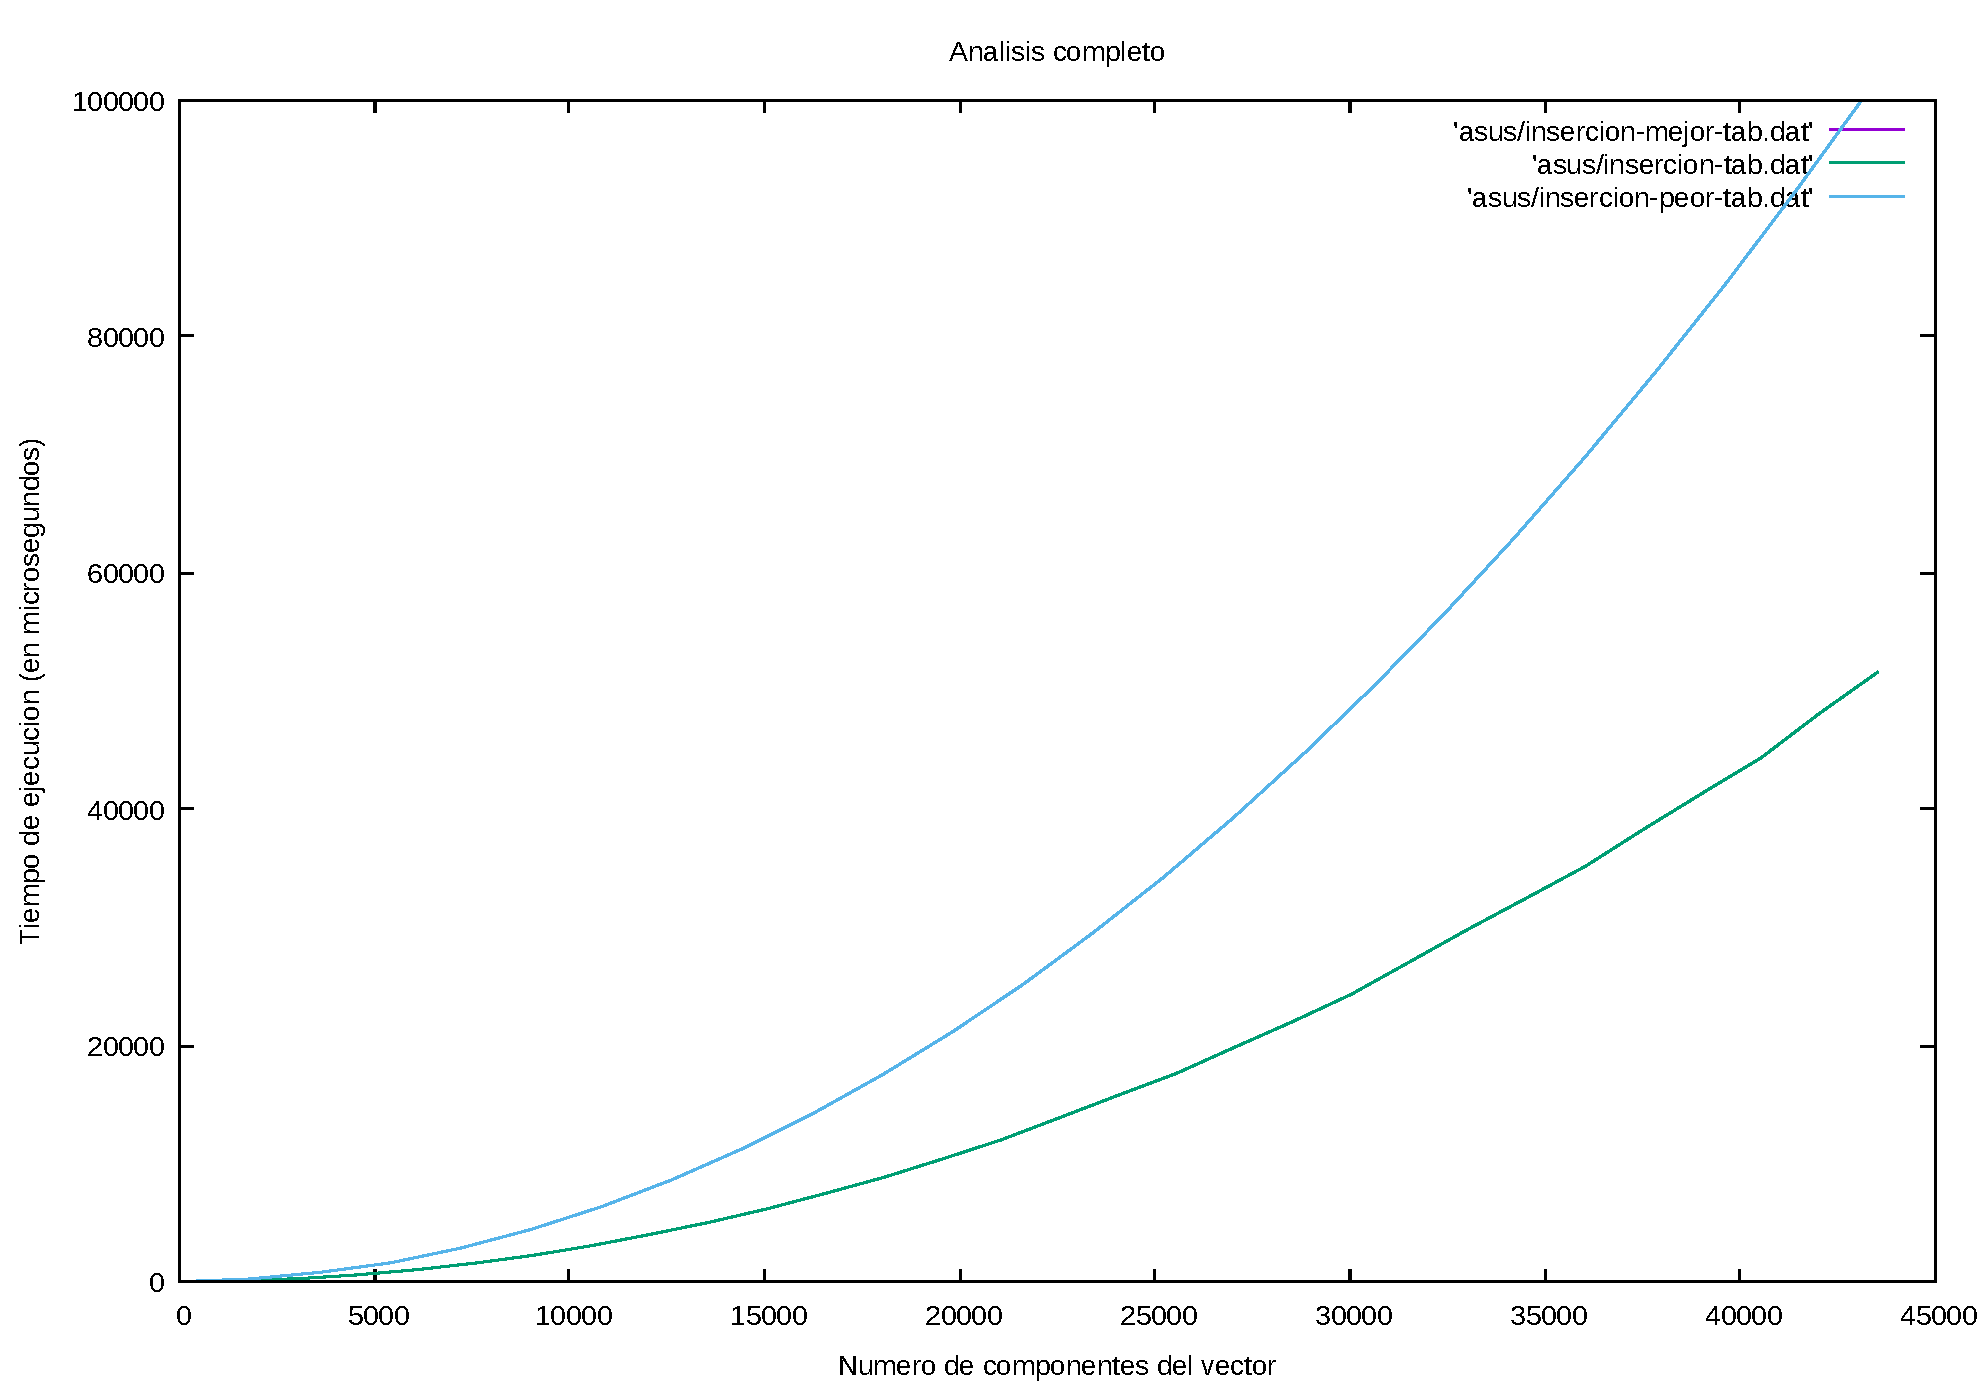
\includegraphics[width=0.67\textwidth]{../data/asus-insercion-mp.pdf}
        \caption{Gráfico de mejor caso, caso promedio y peor caso del algoitmo de Inserción (ASUS)}
    \end{figure}

    \begin{table}[H] 
        \footnotesize
        \centering 
        \begin{tabular}{|r|r|r|r|} 
                \hline
                $N_{\text{componentes}}$ & $T_{\text{mejor}}$ & $T_{\text{prom}}$ & $T_{\text{peor}}$ \\
                \hline  
                5 & 0.08 & 0.18 & 0.10 \\ 
                1807 & 0.26 & 165.44 & 183.66 \\ 
                3609 & 0.42 & 378.04 & 760.00 \\ 
                5410 & 0.80 & 586.46 & 1701.78 \\ 
                7212 & 1.54 & 1038.65 & 3031.90 \\ 
                9014 & 1.92 & 1571.11 & 4605.94 \\ 
                10816 & 2.54 & 2257.82 & 6818.84 \\ 
                12618 & 4.02 & 3038.05 & 9111.40 \\ 
                14419 & 5.08 & 3987.64 & 11713.16 \\ 
                16221 & 5.72 & 5034.40 & 14577.46 \\ 
                18023 & 6.26 & 6111.62 & 17373.86 \\ 
                19825 & 6.90 & 7329.81 & 20950.86 \\ 
                21627 & 8.96 & 8700.77 & 24953.08 \\ 
                23428 & 9.72 & 10203.49 & 29744.30 \\ 
                25230 & 10.06 & 11768.61 & 34166.00 \\ 
                27032 & 10.16 & 13507.03 & 38739.54 \\ 
                28834 & 9.90 & 15368.75 & 43993.08 \\ 
                30636 & 11.04 & 17377.42 & 49710.12 \\ 
                32437 & 12.44 & 19877.53 & 55729.26 \\ 
                34239 & 13.04 & 22049.19 & 62191.36 \\ 
                36041 & 13.48 & 24031.41 & 70366.98 \\ 
                37843 & 14.12 & 26888.22 & 77407.66 \\ 
                39645 & 14.70 & 29816.95 & 83067.28 \\ 
                41446 & 15.42 & 32544.47 & 92339.86 \\ 
                43248 & 15.78 & 34468.33 & 100877.78 \\ 
                \hline
        \end{tabular}
        \caption{Tiempos de ejecución, en $\mu$s, para mejor caso, caso promedio y peor caso (HP) para Inserción}
    \end{table}

    \begin{figure}[H]
        \centering
        \label{hp:insercion-mp}
        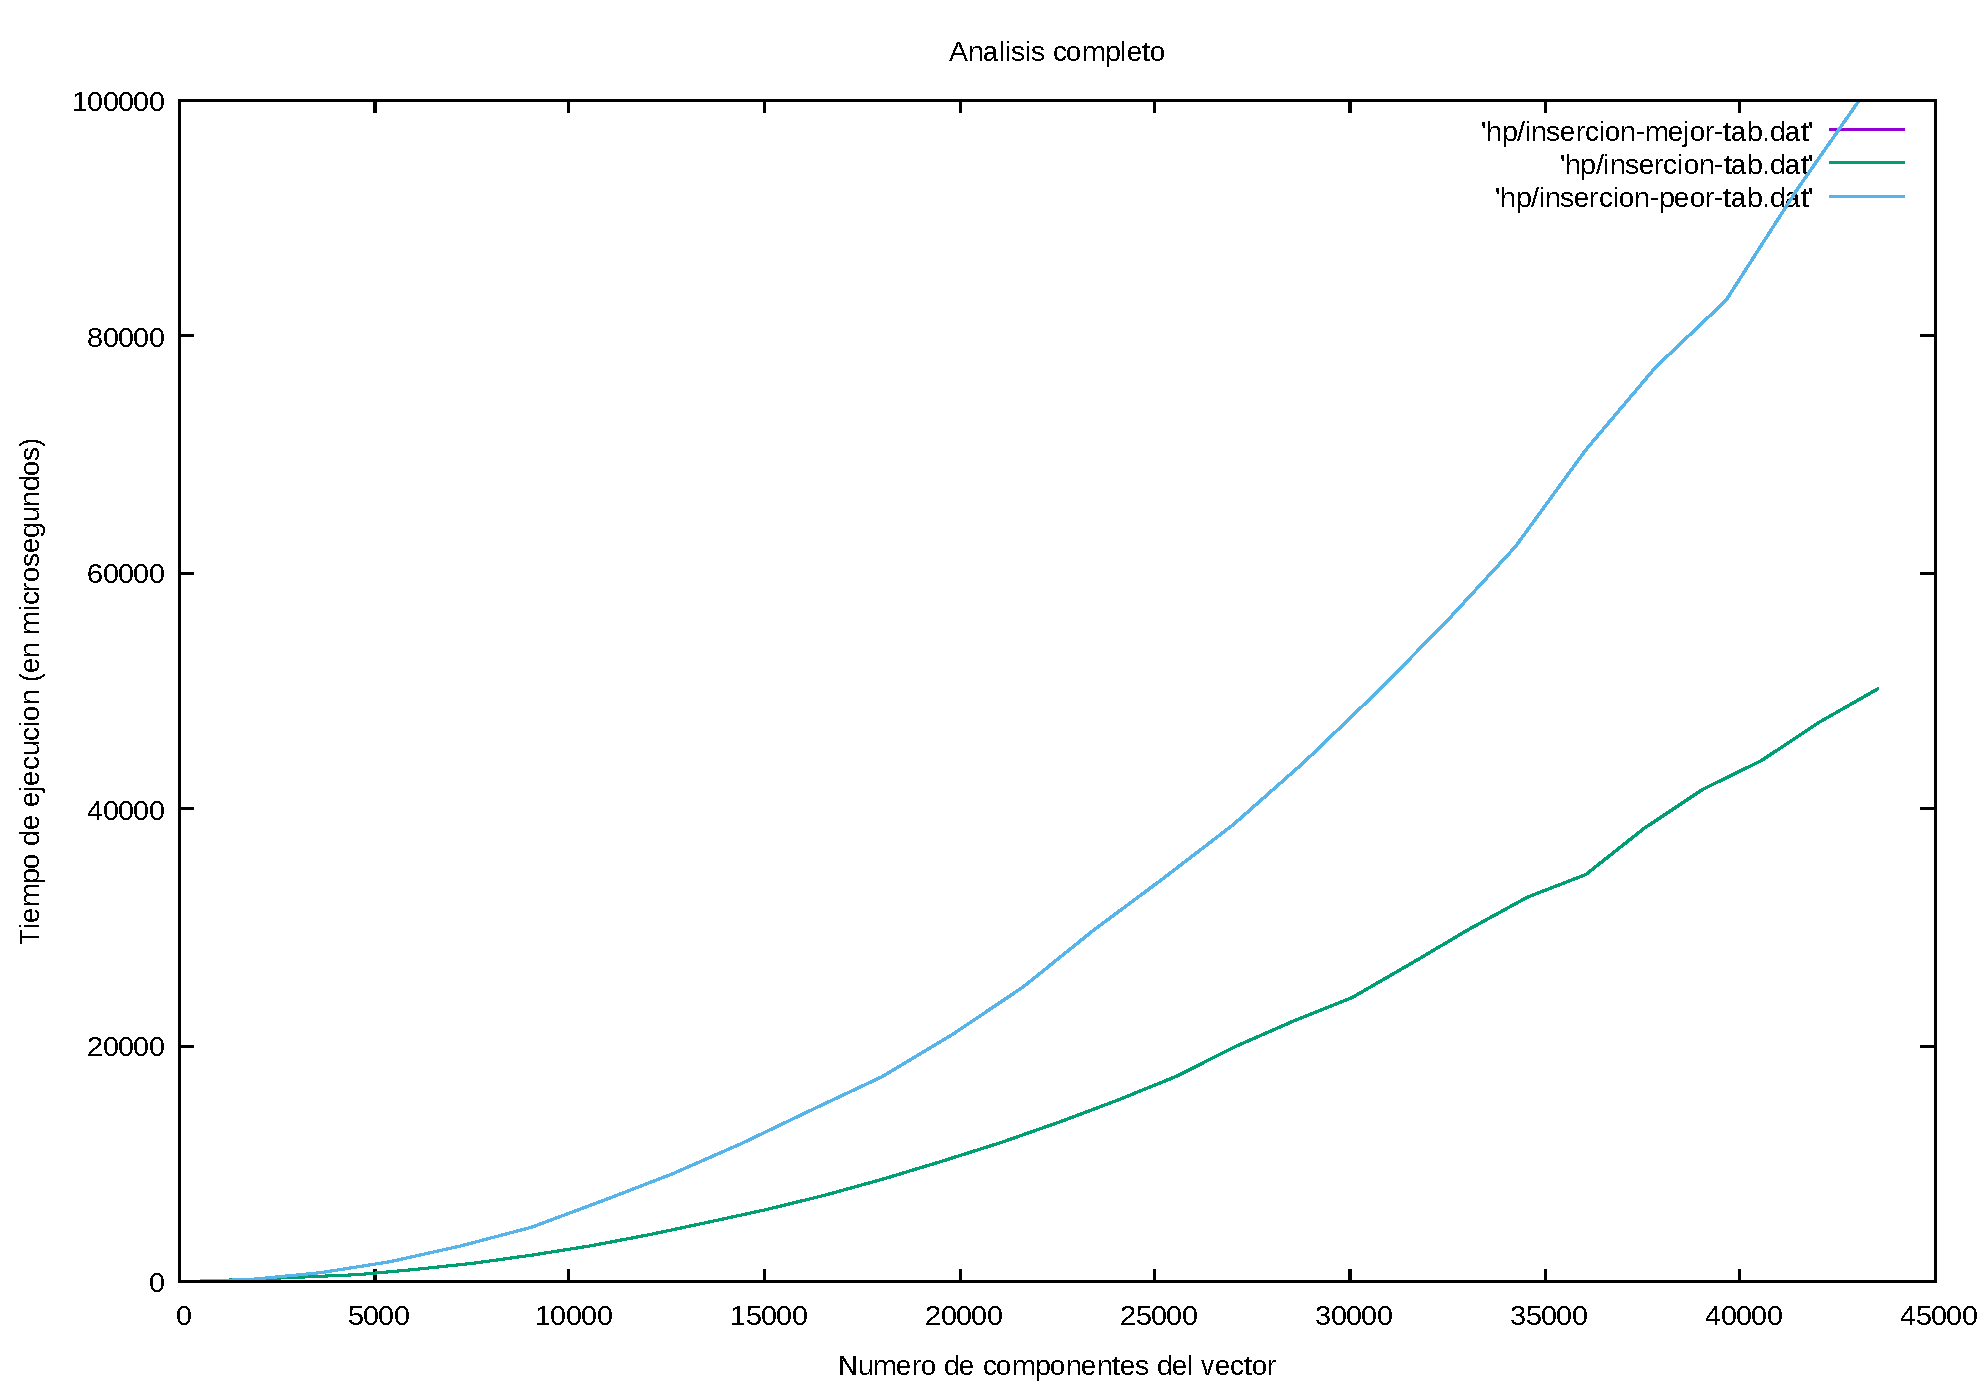
\includegraphics[width=0.67\textwidth]{../data/hp-insercion-mp.pdf}
        \caption{Gráfico de mejor caso, caso promedio y peor caso del algoitmo de Inserción (HP)}
    \end{figure}

    \begin{table}[H] 
        \footnotesize
        \centering 
        \begin{tabular}{|r|r|r|r|} 
                \hline
                $N_{\text{componentes}}$ & $T_{\text{mejor}}$ & $T_{\text{prom}}$ & $T_{\text{peor}}$ \\
                \hline  
                5 & 0.10 & 0.32 & 0.10 \\ 
                1807 & 0.36 & 113.40 & 303.50 \\ 
                3609 & 0.56 & 416.61 & 1108.16 \\ 
                5410 & 0.98 & 818.87 & 2334.58 \\ 
                7212 & 1.54 & 1318.29 & 3649.72 \\ 
                9014 & 1.76 & 2040.42 & 6012.42 \\ 
                10816 & 2.08 & 2893.16 & 8292.62 \\ 
                12618 & 2.52 & 3937.94 & 11154.14 \\ 
                14419 & 2.56 & 5111.43 & 14570.74 \\ 
                16221 & 2.84 & 6412.50 & 18535.08 \\ 
                18023 & 3.20 & 7911.75 & 22866.82 \\ 
                19825 & 4.60 & 9605.05 & 27608.30 \\ 
                21627 & 4.14 & 11396.08 & 32934.78 \\ 
                23428 & 4.04 & 13402.47 & 38583.14 \\ 
                25230 & 4.58 & 15511.25 & 45127.84 \\ 
                27032 & 4.66 & 17763.31 & 54124.70 \\ 
                28834 & 5.40 & 20213.18 & 63231.04 \\ 
                30636 & 5.76 & 22797.11 & 68667.92 \\ 
                32437 & 5.76 & 25575.44 & 74045.08 \\ 
                34239 & 6.14 & 28426.29 & 82508.38 \\ 
                36041 & 6.16 & 31521.96 & 98212.32 \\ 
                37843 & 6.48 & 34782.56 & 103327.70 \\ 
                39645 & 6.80 & 38191.71 & 110208.00 \\ 
                41446 & 8.20 & 41713.63 & 120605.40 \\ 
                43248 & 7.56 & 45353.92 & 130914.20 \\ 
                \hline
        \end{tabular}
        \caption{Tiempos de ejecución, en $\mu$s, para mejor caso, caso promedio y peor caso (Lenovo) para Inserción}
    \end{table}

    \begin{figure}[H]
        \centering
        \label{lenovo:insercion-mp}
           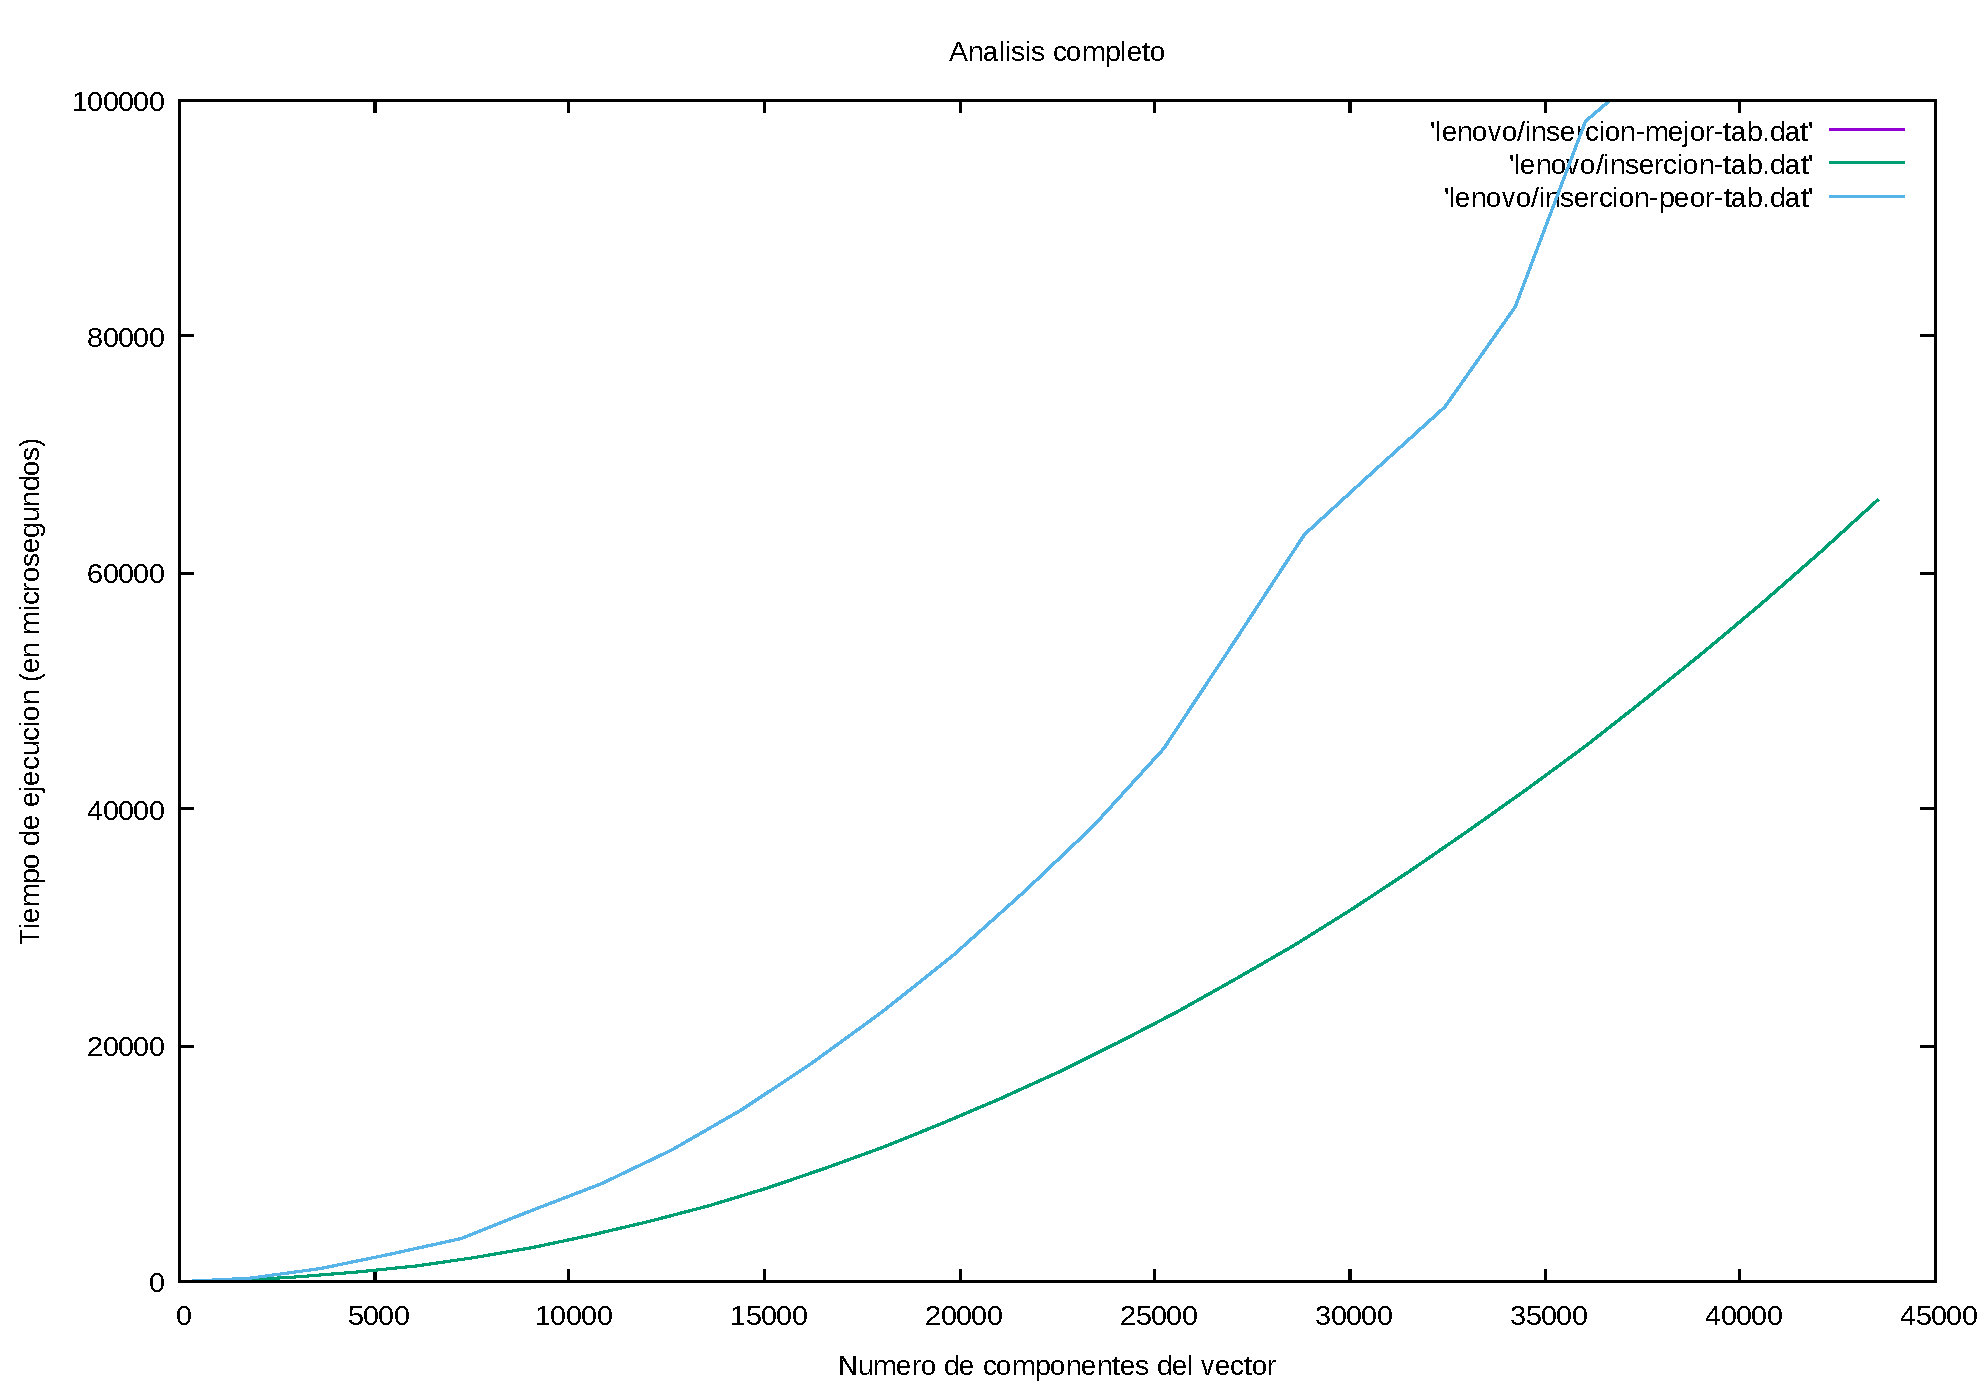
\includegraphics[width=0.67\textwidth]{../data/lenovo-insercion-mp.pdf}
        \caption{Gráfico de mejor caso, caso promedio y peor caso del algoitmo de Inserción (Lenovo)}
    \end{figure}

    \subsection{Análisis}

    Como podemos observar, como cabía esperar el caso promedio se sitúa entre el mejor y el peor caso de ejecución
    de los algoritmos. Vemos que tanto el mejor y el peor caso tienen el mismo orden de eficiencia que el caso promedio
    por lo que para el análisis teórico anterior podríamos haber incluso empleado la notación $\theta (n)$ (si bien no
    se ha incluido para evitar hacer esta memoria demasiado larga). 
    
    También es un hecho destacable que, en el caso del algoritmo de Inserción, el mejor caso presenta un muy buen
    comportamiento en el mejor caso, pero para el peor caso se ralentiza considerablemente, puesto que presenta
    un tiempo de ejecución muy superior al algoritmo de Selección. En el caso promedio ambos presentan un comportamiento
    muy parecido, por lo podemos extraer las siguientes conclusiones:
    
    \begin{itemize}
        \item Para situaciones en los que es más probable que se presenten los datos ordenados en orden creciente, tenemos que el algoritmo óptimo es Inserción (pues en el mejor caso presenta un comportamiento lineal). 
        \item Para situaciones en los que es más probable encontrar datos desordenados, ambos algoritmos se comportan de forma similar. 
        \item Cuando se ejecute el algoritmo Inserción, es más conveniente comprobar previamente que la estructura de datos no esté ordenado en forma decreciente.
    \end{itemize}
    
    En cualquier caso, para pequeños valores de los componentes de los vectores la diferencia en rendimiento es prácticamente despreciable, por
    lo que ambos algoritmos son igual de válidos para estas situaciones y debería prevalecer más otros factores ajenos a su eficiencia.

    \newpage
    \section{Eficiencia híbrida} 
    
    En esta sección trataremos los datos obtenidos de la sección anterior mediante técnicas estadísticas para
    comprobar la consistencia de los datos experimentales con los calculados teóricamente. 

    \subsection{Comparación entre diferentes tipos de ajustes}

    Para esta sección, hemos hecho uso del GraphKiller, el cual ha ejecutado automáticamente todas las posibles regresiones
    que se pueden presentar en esta práctica y se ha seleccionado de, entre ellas, la regresión que mejor se ajusta a los datos
    experimentales. Un ejemplo de ello lo podemos ver en los siguientes ficheros, generador por cada ordenador para el algoritmo de Floyd 
    (las regresiones que no aparecen son debido a que generar error en la ejecución de Gnuplot, por lo que GraphKiller opta por no
    incluirlo en este fichero):

    \lstinputlisting[caption=Fichero de salida generado por GraphKiller en ASUS]{../data/asus/floyd-general-stat.txt}
    \lstinputlisting[caption=Fichero de salida generado por GraphKiller en HP]{../data/hp/floyd-general-stat.txt}
    \lstinputlisting[caption=Fichero de salida generado por GraphKiller en Lenovo]{../data/lenovo/floyd-general-stat.txt}

    El dato que más nos puede interesar es RMS, que proporciona una medida del nivel de ajuste conseguido por la curva de regresión,
    de forma que cuanto menor sea su valor mejor es el ajuste conseguido. 

    De esta manera, hemos comprobado para cada uno de los algoritmos presentes en esta práctica cada una de las regresiones, 
    y hemos seleccionado seleccionado el mejor ajuste en cada uno de ellos (que coinciden con el predicho teóricamente, como veremos
    más adelante). Por simplicidad, hemos optado por no incluir todos los parámetros de regresión obtenidos. 

    \subsection{Algoritmo QuickSort}

    Las gráficas con las curvas de regresión son las que se obtienen en las imágenes \ref{hib:quicksort}.

    \begin{figure}
        \centering
         \subfloat[ASUS]{
          \label{asus:quicksort-hib}
           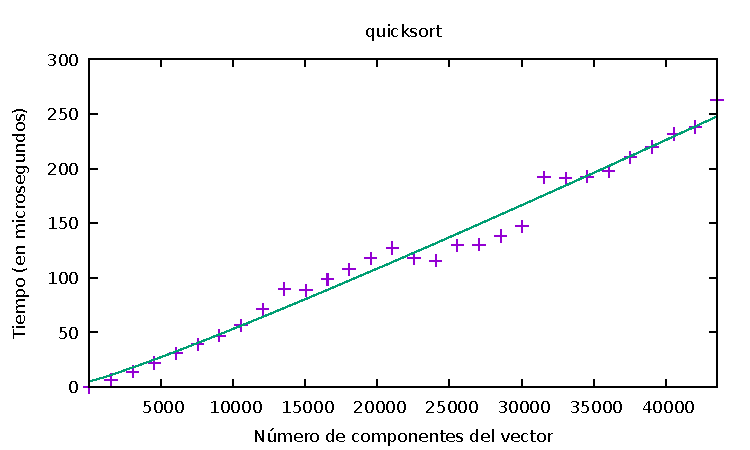
\includegraphics[width=0.7\textwidth]{../data/asus/quicksort-graph.pdf}}

         \subfloat[HP]{
          \label{hp:quicksort-hib}
           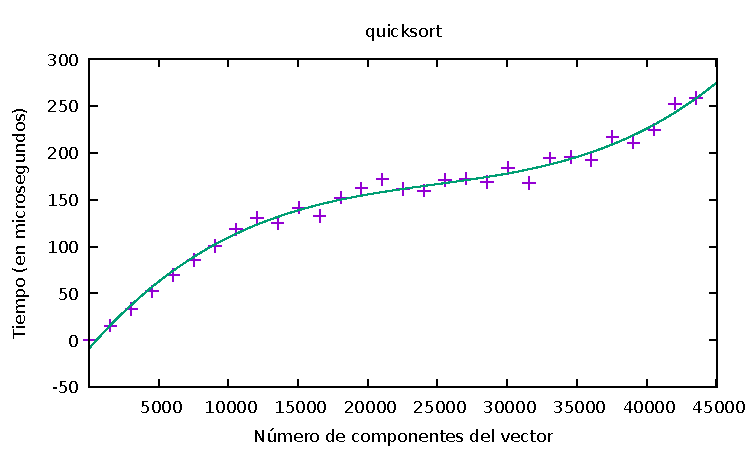
\includegraphics[width=0.7\textwidth]{../data/hp/quicksort-graph.pdf}}

         \subfloat[LENOVO]{  
          \label{lenovo:quicksort-hib}
           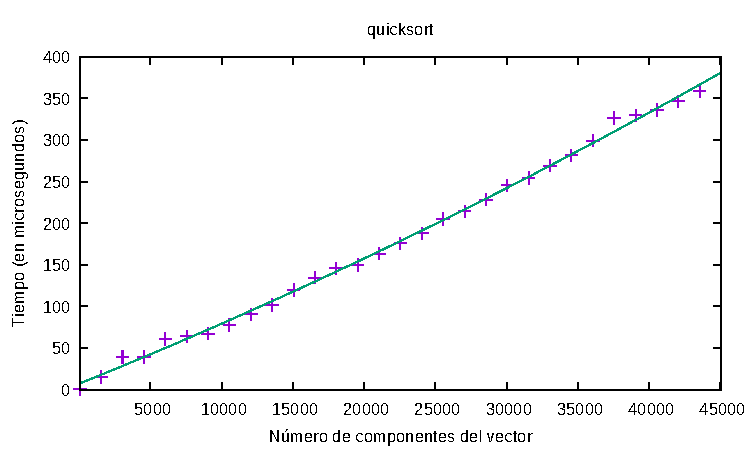
\includegraphics[width=0.7\textwidth]{../data/lenovo/quicksort-graph.pdf}}
        \caption{Gráficas de regresión de los algoritmos de QuickSort.}

        \label{hib:quicksort}
    \end{figure}

    De acuerdo con lo calculado previamente, veamos si la regresión superlineal es un buen ajuste. Mediante técnicas estadísticas
    obtenemos los siguientes valores de regresión en cada uno de los equipos:

    \begin{table}[H]
        \centering
        \begin{tabular}{|c|c|c|}
            \hline
            Equipo & Función de regresión & Coeficiente de determinación \\
            \hline
            Asus & $5.10 \cdot 10^{-4} x \log(x) + 5.112$ & $0.9798$ \\
            HP & $3.66 \cdot 10^{-4} x \log(x) + 50$ & $0.9957$ \\
            Lenovo & $7.72 \cdot 10^{-4} x \log(x) + 5.423$ & $0.9969$ \\
            \hline
        \end{tabular}
        \caption{Funciones de ajuste del algoritmo QuickSort en diferentes equipos}
    \end{table}

    \subsection{Algoritmo de inserción}

    Las gráficas con las curvas de regresión son las que se obtienen en las imágenes \ref{hib:insercion}.

    \begin{figure}
        \centering
         \subfloat[ASUS]{
          \label{asus:insercion-hib}
           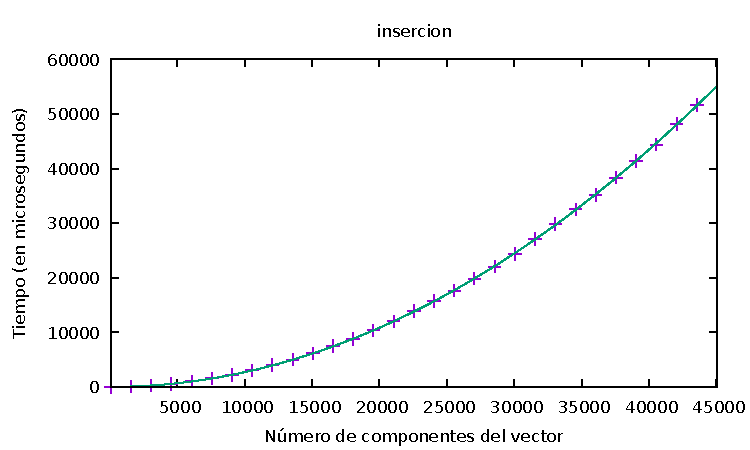
\includegraphics[width=0.7\textwidth]{../data/asus/insercion-graph.pdf}}

         \subfloat[HP]{
          \label{hp:insercion-hib}
           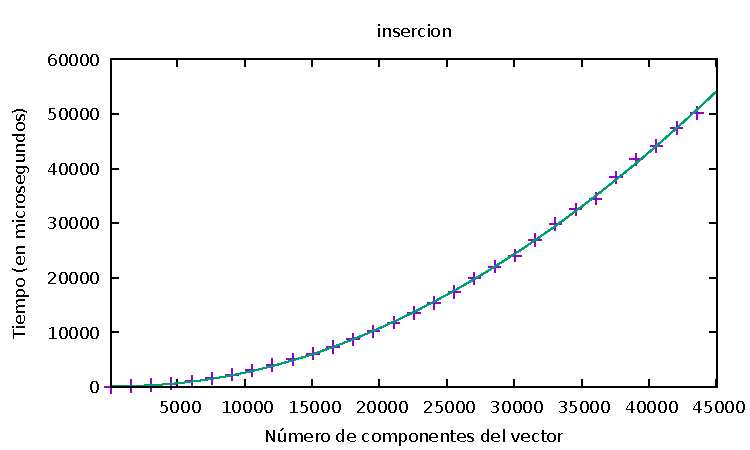
\includegraphics[width=0.7\textwidth]{../data/hp/insercion-graph.pdf}}

         \subfloat[LENOVO]{
          \label{lenovo:insercion-hib}
           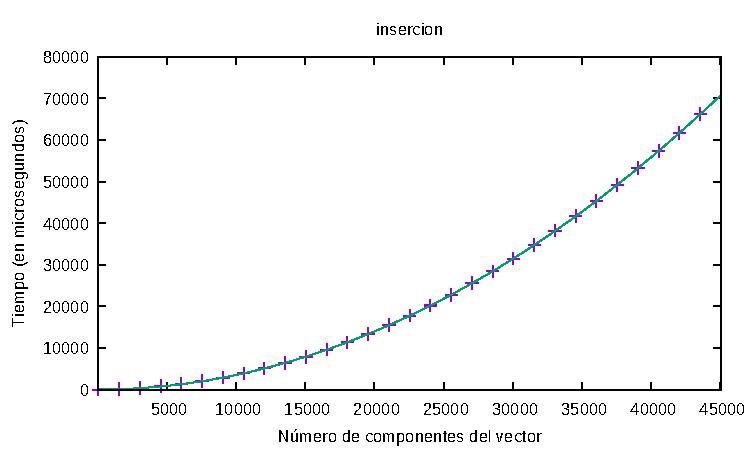
\includegraphics[width=0.7\textwidth]{../data/lenovo/insercion-graph.pdf}}
        \caption{Gráficas de regresión de los algoritmos de Inserción.}

        \label{hib:insercion}
    \end{figure}

    Para cada una de ellas se han obtenido los datos de la tabla \ref{insercion:tab}. 

    \begin{table}[H]
        \centering
        \begin{tabular}{|c|c|c|}
            \hline
            Equipo & Función de regresión & Coeficiente de determinación \\
            \hline
            Asus & $2.7192 \cdot 10^{-5} x^2 - 0.00212952 x + 22.2497$ & $1.0000$ \\
            HP & $2.69268 \cdot 10^{-5} x^2 - 0.0250169 x + 353.105$ &  $1.0000$ \\
            Lenovo & $3.48955 \cdot 10^{-5} x^{2} - 0.000620098 x + 48.0855$ & $1.0000$ \\
            \hline
        \end{tabular}
        \caption{Funciones de ajuste del algoritmo de Inserción en diferentes equipos}
        \label{insercion:tab}
    \end{table} 

    Por tanto, como en los tres casos el coeficiente de determinación es 1, el ajuste para el algoritmo de Inserción 
    usando una función cuadrática es perfecto.

    \subsection{Algoritmo Floyd}

    Las gráficas con las curvas de regresión son las que se obtienen en las imágenes \ref{hib:floyd}.

    \begin{figure}
        \centering
         \subfloat[ASUS]{
          \label{asus:floyd-hib}
           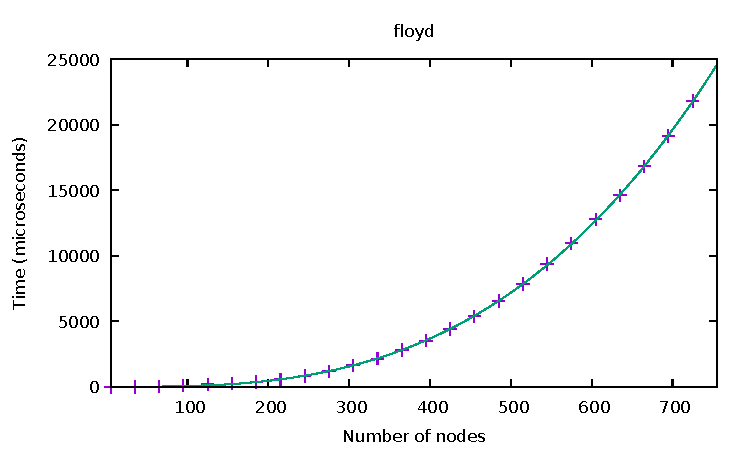
\includegraphics[width=0.7\textwidth]{../data/asus/floyd-graph.pdf}}

         \subfloat[HP]{
          \label{hp:floyd-hib}
           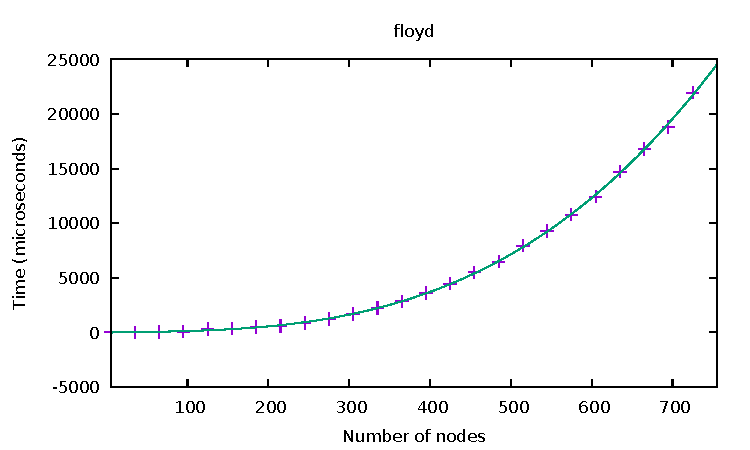
\includegraphics[width=0.7\textwidth]{../data/hp/floyd-graph.pdf}}

         \subfloat[LENOVO]{  
          \label{lenovo:floyd-hib}
           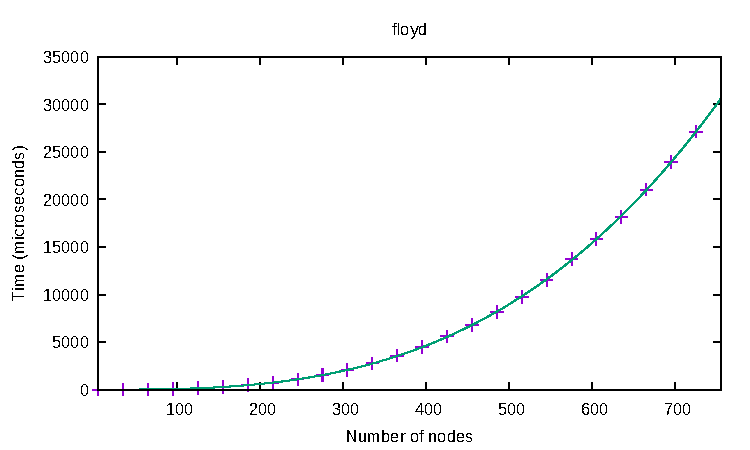
\includegraphics[width=0.7\textwidth]{../data/lenovo/floyd-graph.pdf}}
        \caption{Gráficas de regresión de los algoritmos de Floyd.}

        \label{hib:floyd}
    \end{figure}

    Para cada una de ellas se han obtenido los siguientes datos:

    \begin{table}[H]
        \centering
        \begin{tabular}{|c|c|c|}
            \hline
            Equipo & Función de regresión & Coeficiente de determinación \\
            \hline
            Asus & $5.57676 \cdot 10^{-5} x^3 + 0.00138722 x^2-0.315202 x + 34.0467$ & $1.0000$ \\
            HP & $5.96848 \cdot 10^{-5} x^3 - 0.00353189 x^2 + 1.17214 x - 20.9986$ & $0.9997$ \\
            Lenovo & $6.96669 \cdot 10^{-5} x^3 + 0.00112974 x^2 - 0.00362409 x + 0.857106$ & $1.0000$ \\
            \hline
        \end{tabular}
        \caption{Funciones de ajuste del algoritmo de Floyd en diferentes equipos}
    \end{table}

    Por tanto, como en los tres casos el coeficiente de determinación es 1, el ajuste para el algoritmo Floyd 
    usando una función cúbica es perfecto.

    \subsection{Algoritmo Hanoi}

    Las gráficas con las curvas de regresión son las que se obtienen en las imágenes \ref{hib:hanoi}.

    \begin{figure}
        \centering
         \subfloat[ASUS]{
          \label{asus:hanoi-hib}
           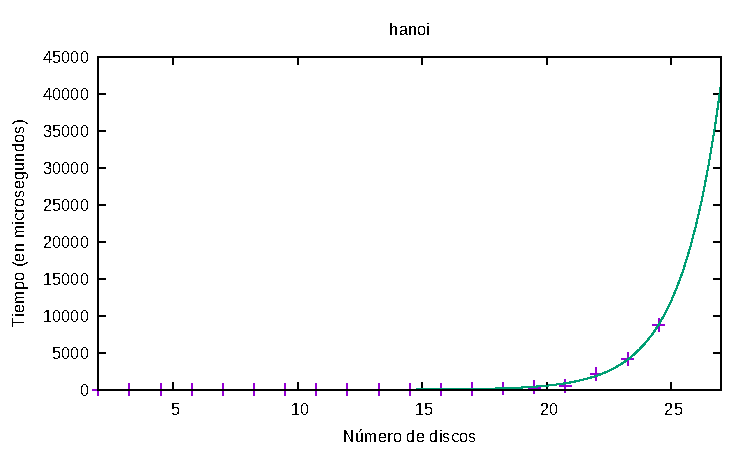
\includegraphics[width=0.7\textwidth]{../data/asus/hanoi-graph.pdf}}

         \subfloat[HP]{
          \label{hp:hanoi-hib}
           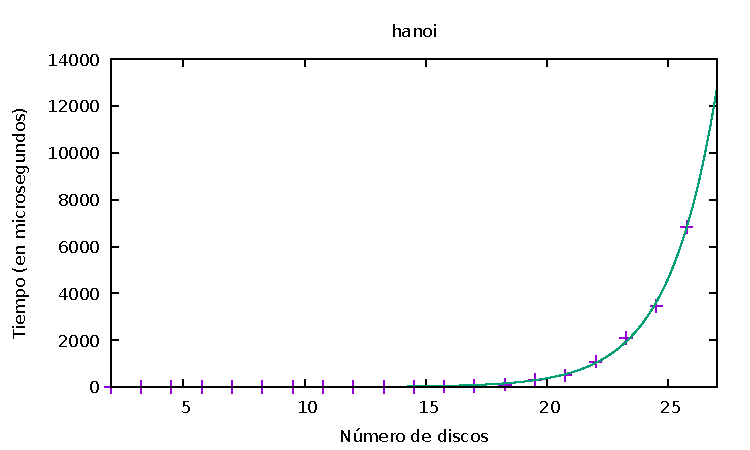
\includegraphics[width=0.7\textwidth]{../data/hp/hanoi-graph.pdf}}

         \subfloat[LENOVO]{  
          \label{lenovo:hanoi-hib}
           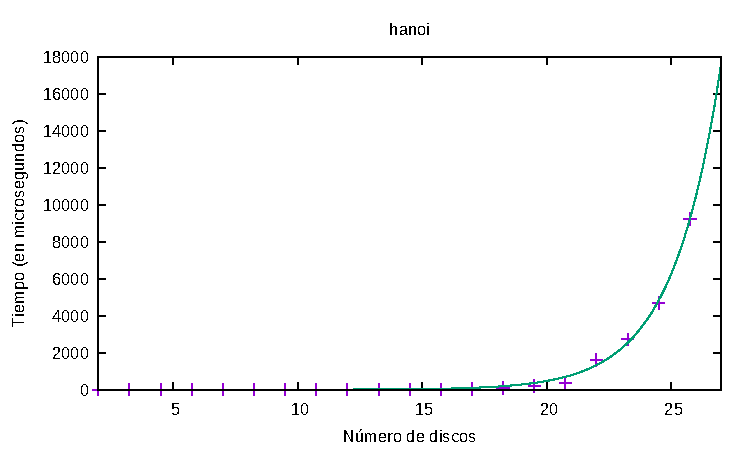
\includegraphics[width=0.7\textwidth]{../data/lenovo/hanoi-graph.pdf}}
        \caption{Gráficas de regresión de los algoritmos de Floyd.}

        \label{hib:hanoi}
    \end{figure}

    Para cada una de ellas se han obtenido los siguientes datos:

    \begin{table}[H]
        \centering
        \begin{tabular}{|c|c|c|}
            \hline
            Equipo & Función de regresión & Coeficiente de determinación \\
            \hline
            Asus & $0.00231633 \cdot e^{0.618424 x}$ & $0.9892$ \\
            HP & $0.0158 \cdot e^{0.503814 x}$ & $0.9921$ \\
            Lenovo & $0.0153331 \cdot e^{0.516756 x}$ & $0.9765$ \\
            \hline
        \end{tabular}
        \caption{Funciones de ajuste del algoritmo de Hanoi en diferentes equipos}
    \end{table}

    Por tanto, como en los tres casos el coeficiente de determinación muestra una gran cercanía al 1, el ajuste para el algoritmo Hanoi 
    usando una función exponencial es bastante razonable, lo que confirma nuestros cálculos previos que nos indican que su eficiencia es 
    exponencial.

    \newpage
    
    \section{Conclusión}

    La Algorítmica trata el estudio profundo y exhaustivo de los algoritmos, que constituyen la pieza clave para   
    la resolución de problemas de diferente naturaleza que pueden modelarse de manera computacional. De ahí la importancia 
    de su análisis, que consiste en dado un problema del cual disponemos de varios algoritmos para su resolución,
    encontrar el mejor algoritmo que resuelve ese problema. La elección del mejor algoritmo depende del criterio que 
    consideremos, de los cuales podemos destacar la adaptibilidad del algoritmo a los computadores, su simplicidad, el costo 
    económico de su confección, y la duración del tiempo consumido para llevar a cabo el algoritmo. 
    
    El último criterio mencionado es el que se ha desarrollado en esta práctica, la cual ha consistido en analizar la eficiencia
    de seis algoritmos, cuatro de ellos modelan el mismo problema, la ordenación de vectores de datos numéricos, uno resuelve el problema
    de las torres de Hanoi y el otro resuelve el problema de encontrar caminos mínimos en grafos, conocido como algoritmo de Floyd. 
    
    Nuestro trabajo ha consistido en determinar la eficiencia teórica de cada uno de los algoritmos propuestos, y la eficiencia empírica calculando
    el tiempo de ejecución para diferentes tamaños de problema. Así, hemos tratado de de dar respuesta a los distintos objetivos planteados al inicio
    de esta memoria:

    Uno de ellos consistía en verificar si los análisis empíricos verifican o no los resultados teóricos esperados. Una vez obtenidos los datos 
    referentes al tiempo de ejecución segun el tamaño del problema, hemos tratado de ajustar dichos datos experimentales con funciones de regresión de 
    distinto tipo (constante, sublineal, logaritmico, lineal, supralineal, cuadrático y cúbico), y calculado los coeficientes de determinación correspondientes
    a dicho ajuste. De este modo, hemos podido comprobar que la función de regresión que mejor se ajusta en cada caso coincide con el tipo de función
    obtenida con el análisis teórico asintótico big O, de tal forma que para algoritmos como Inserción o Floyd el ajuste es perfecto (el coeficiente de 
    determinación es uno). Esta tarea la hemos llevado a cabo en diferentes equipos (Asus, HP y Lenovo), y hemos podido comprobar que los tiempos de 
    ejecución de cada algoritmo mejoran cuando las prestaciones hardware de los equipos son de mayor calidad, poniendo de manifiesto la importancia de conocer
    el hardware de los equipos para poder determinar la viabilidad en cuanto a la ejecución de los algoritmos en los diferentes equipos. 

    También, para dar respuesta al problema de la elección de un algoritmo, hemos usado el problema de la ordenación, para el cual teniamos cuatro 
    opciones disponibles. Hemos concluido el tiempo de ejecución es menor para algoritmos con mejores ordenes de eficiencia, por lo que conviene su 
    uso para grandes tamaños de problemas, también hemos observado que para tamaños pequeños el rendimiento es casi el mismo, lo cual ejemplifica la
    necesidad de conocer el contexto de ejecución de cada uno de los algoritmos para lograr una mejor adaptabilidad a las opciones que tengamos disponibles.
    También hemos analizado el caso más favorable y desfavorable del conjunto de datos para los algoritmos de Inserción y Selección, el tiempo de ejecución se 
    reduce considerablemente en vectores ordenados ascendentemente, y aumenta en vectores ordenados descendentemente, aumentando dicho contraste en Inserción. 
    
    Por último, hemos de destacar el estudio realizado para distintas optimizaciones del compilador g++. Los algoritmos son independientes de las distintas
    implementaciones que podamos hacer de ellos en distintos lenguajes de programación, pero hemos de comprender que en la práctica entender el comportamiento
    de las herramientas que usamos es fundamental para poder llegar a resultados sólidos y congruentes. Es por ello por lo que realizamos este estudio, empleando 
    el algoritmo de Floyd para ello, y hemos concluido que las distintas optimizaciones con las que podamos compilar un mismo programa influyen considerablemente en el tiempo de ejecución en todos los 
    equipos empleados para tamaños de problema elevados, siendo la diferencia especialmente notable entre los casos en los que no usamos optimización y entre los que sí lo hacemos.
    
    En definitiva, esta práctica nos ha servido para entender el papel fundamental de la Algoritmica en la búsqueda de la mejor opción para resolver un problema
    computacional, y nos sirve de base para entender el contexto y motivar los conceptos que aprenderemos en esta asignatura.

    \newpage
    \begin{thebibliography}{0}
        \bibitem{Verdegay2017} Verdegay Galdeano. (2017). Lecciones de Algorítmica / José Luis Verdegay. Técnica Avicam.
        \bibitem{Cormen2017} Cormen. (2017). Introduction to algorithms / Thomas H. Cormen... [et al.] (3rd ed.). PHI Learning.
        \bibitem{Garrido2018} Garrido Carrillo. (2018). Estructuras de datos avanzadas: con soluciones en C++ / A. Garrido. Universidad de Granada.        
    \end{thebibliography}
    

\end{document} 